\documentclass[enabledeprecatedfontcommands,fontsize=12pt,paper=a4,twoside]{scrartcl}


\newcommand{\grad}{\ensuremath{^{\circ}} }
\renewcommand{\strut}{\vrule width 0pt height5mm depth2mm}

\usepackage{longtable}
\usepackage[utf8]{inputenc}
\usepackage[T1]{fontenc}
\usepackage[final]{pdfpages}
% obere Seitenränder gestalten können
\usepackage{fancyhdr}
\usepackage{moreverb}
% Graphiken als jpg, png etc. einbinden können
\usepackage{graphicx}
\usepackage[normalem]{ulem}
\useunder{\uline}{\ul}{}
\usepackage{stmaryrd}
% Floats Objekte mit [H] festsetzen
\usepackage{float}
% setzt URL's schön mit \url{http://bla.laber.com/~mypage}
\usepackage{url}
% Externe PDF's einbinden können
\usepackage{pdflscape}
% Verweise innerhalb des Dokuments schick mit " ... auf Seite ... "
% automatisch versehen. Dazu \vref{labelname} benutzen
\usepackage[ngerman]{varioref}
\usepackage[ngerman]{babel}
\usepackage{ngerman}
% Bibliographie
\usepackage{bibgerm}
% Tabellen
\usepackage{tabularx}
\usepackage{supertabular}
\usepackage[colorlinks=true, pdfstartview=FitV, linkcolor=blue,
            citecolor=blue, urlcolor=blue, hyperfigures=true,
            pdftex=true]{hyperref}
\usepackage{bookmark}
\usepackage{rotating}
\usepackage{float}

\hyphenation{Arbeits-paket}

% Damit Latex nicht zu lange Zeilen produziert:
\sloppy
%Uneinheitlicher unterer Seitenrand:
%\raggedbottom

% Kein Erstzeileneinzug beim Absatzanfang
% Sieht aber nur gut aus, wenn man zwischen Absätzen viel Platz einbaut
\setlength{\parindent}{0ex}

% Abstand zwischen zwei Absätzen
\setlength{\parskip}{1ex}

% Seitenränder für Korrekturen verändern
\addtolength{\evensidemargin}{-1cm}
\addtolength{\oddsidemargin}{1cm}

\bibliographystyle{gerapali}

% Lustige Header auf den Seiten
  \pagestyle{fancy}
  \setlength{\headheight}{70.55003pt}
  \fancyhead{}
  \fancyhead[LO,RE]{Software--Projekt 2\\ WiSe 2019/2020
  \\Architekturbeschreibung}
  \fancyhead[LE,RO]{Seite \thepage\\\slshape \leftmark\\\slshape \rightmark}

%Unicode Minuszeichen deklarieren, um es nicht überall austauschen zu müssen
\DeclareUnicodeCharacter{2212}{-}

%
% Und jetzt geht das Dokument los....
%

\begin{document}

% Lustige Header nur auf dieser Seite
  \thispagestyle{fancy}
  \fancyhead[LO,RE]{ }
  \fancyhead[LE,RO]{Universität Bremen\\FB 3 -- Informatik\\
  Prof. Dr. Rainer Koschke \\TutorIn: Marcel Steinbeck}
  \fancyfoot[C]{}

% Start Titelseite
  \vspace{3cm}

  \begin{minipage}[H]{\textwidth}
  \begin{center}
  \bf
  \Large
  Software--Projekt 2 WiSe 2019/2020\\
  \smallskip
  \small
  VAK 03-BA-901.02\\
  \vspace{3cm}
  \end{center}
  \end{minipage}
  \begin{minipage}[H]{\textwidth}
  \begin{center}
  \vspace{1cm}
  \bf
  \Large Benutzerhandbuch\\ Data Colorado\\
  \vfill
  \end{center}
  \centering
  
\includegraphics[width=0.4\textwidth]{UML/Logo.png}\\
  \end{minipage}
  \vfill
  \begin{minipage}[H]{\textwidth}
  \begin{center}
  \sf
  \begin{tabular}{lr}
  Liam Hurwitz & hurwitz@tzi.de \\
  Kevin Santiago Rodriguez Rey & kev\textunderscore rey@tzi.de \\
  Fabian Kehlenbeck & fkehlenb@tzi.de \\
  Aaron Rudkowski & rudkowsk@tzi.de \\
  Samuel Nejati Masouleh & samnej@tzi.de \\
  Leonard Haddad & s\textunderscore xsipo6@tzi.de \\  
\end{tabular}
  \\ ~
  \vspace{2cm}
  \\
  \it Abgabe: 08.03.2020 --- Version 1.0\\ ~
  \end{center}
  \end{minipage}

% Ende Titelseite

% Start Leerseite

\newpage

  \thispagestyle{fancy}
  \fancyhead{}
  \fancyhead[LO,RE]{Software--Projekt \\  2019/2020
  \\Benutzerhandbuch}
  \fancyhead[LE,RO]{Seite \thepage\\\slshape \leftmark\\~}
  \fancyfoot{}
  \renewcommand{\headrulewidth}{0.4pt}
  \tableofcontents

\newpage

  \fancyhead[LE,RO]{Seite \thepage\\\slshape \leftmark\\\slshape \rightmark}


%%%%%%%%%%%%%%%%%%%%%%%%%%%%%%%%%%%%%%%%%%%%%%%%%%%%%%%%%%%%%%%%%%%%%%%%


\section*{Version und Änderungsgeschichte}

{\em Die aktuelle Versionsnummer des Dokumentes sollte eindeutig und gut zu
identifizieren sein, hier und optimalerweise auf dem Titelblatt.}

\begin{tabular}{ccl}
Version & Datum & Änderungen \\
\hline
%0.1 & TT.MM.JJJJ & Dokumentvorlage als initiale Fassung kopiert \\
0.1 & 03.03.2020 & Erste Schritte \\
0.2 & 03.03.2020 & Administrator \\
0.3 & 04.03.2020 & Prozesskettenadministrator \\
0.4 & 06.03.2020 & Restliche Rollen ohne Screenshots \\
0.5 & 07.03.2020 & Screenshots \\
0.6 & 07.03.2020 & Index, Glossar, Einführung \\
0.7 & 08.03.2020 & Fehlermeldungen \\
\end{tabular}

%%%%%%%%%%%%%%%%%%%%%%%%%%%%%%%%%%%%%%%%%%%%%%%%%%%%%%%%%%%%%%%%%%%%%%%%

\newpage
\section{Einführung}
\subsection{Adressierte Leser}
Die Leser dieses Handbuchs sind alle Benutzer des Systems, was explizit die Beschäftigten des Sonderfachbereichs 1232 Farbige Zustände sind. Diese Beschäftigten können das System zur Organisation der Arbeit in ihrem Fachbereich benutzen. \\
\subsection{Zweck}
Dieses Handbuch soll alle Interaktionen, die mit dem im Rahmen des Softwareprojekt-Kurses von Rainer Koschke entstandenen Software möglich sind, erläutern. Neben den alltäglichen Aktionen mit dem System wird ebenfalls in diesem Dokument die Erstinstallation der Software für den Systemadministrator beschrieben. \\
\subsection{Verwandte Dokumente}
In diesem Dokument wird auf die bis Dezember erstellt Architekturbeschreibung Bezug genommen. \\
\subsection{Konventionen}
\subsection{Information über die Verwendung des Dokuments}
Der Hauptteil des Handbuchs ist nach den im System möglichen Rollen eines Benutzers unterteilt. Im Inhaltsverzeichnis finden Sie die Oberpunkte Administrator (siehe Kapitel 4) sowie Restliche Benutzer des Systems (siehe Kapitel 5 des Systems), was Technologen, Logistiker, Prozessketten Administrator und Transporter sind. Dadurch können Sie sofort den Bereich finden, in dem Sie nach Anleitungen zu Ihren Anliegen suchen. Darüber hinaus gibt es einen Abschnitt für Erstbenutzer des Systems, der einen Überblick über die allgemeinen, rollenunspezifischen Funktionen gibt (siehe Kapitel 3). Falls Sie Erklärungen zu Fehlermeldungen suchen, können Sie diese am Ende von dem rollenspezifischen Unterabschnitt in Kapitel 3 und 4 finden, dessen Funktionen die Meldung ausgelöst haben. \\
Sie können zur einfacheren Bedienung direkt im Inhaltsverzeichnis, sowie bei jeglichen anderen Erwähnungen von Kapiteln, auf die jeweiligen Abschnitte klicken. \\
\subsection{Instruktionen für Problemberichte}

%%%%%%%%%%%%%%%%%%%%%%%%%%%%%%%%%%%%%%%%%%%%%%%%%%%%%%%%%%%%%%%%%%%%%%%%

\newpage
\section{Übersicht}
\subsection{Zugrunde liegende Konzepte, Einbettung}
\subsection{Funktionale Beschreibung}
Farbige Zustände ist eine Webanwendung für die Abläufe im Labor des SFB...\\
In unserer Anwendung haben Benutzer entsprechend Ihrer Rollen eine Übersicht über die Arbeit, die für Sie im Labor anfallen, und können ... \\
\subsection{Gefahren und Warnungen}

%%%%%%%%%%%%%%%%%%%%%%%%%%%%%%%%%%%%%%%%%%%%%%%%%%%%%%%%%%%%%%%%%%%%%%%%

\newpage
\section{Erste Schritte für Anwender}

Im Folgenden werden die grundlegenden Funktionen des Systems für alle Benutzer beschrieben. \\

\subsection{Anmeldung}
Von der Willkommensseite können Sie durch Klicken auf den Link zum Anmeldeformular zu kommen. \\

\begin{figure}[h!]
\begin{center}
 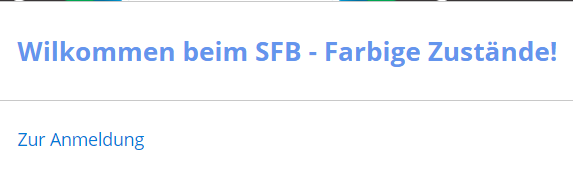
\includegraphics[width=\textwidth]{screenshots/allgemein/willkommen.png}
  \caption{Die Willkommensseite der Anwendung}
  \label{fig:boat1}
\end{center}
\end{figure}

In diesem Formular geben Sie den Namen und das Passwort ein; diese Informationen wurden bei Ihrer Registration festgelegt. Mit Klicken auf Anmelden werden diese Daten überprüft, und wenn sie korrekt sind, werden Sie angemeldet. Weitere Informationen über die Funktionen des Systems finden Sie in den Abschnitten zu den Rollen, denen Sie zugewiesen sind. \\

\begin{figure}[h!]
\begin{center}
 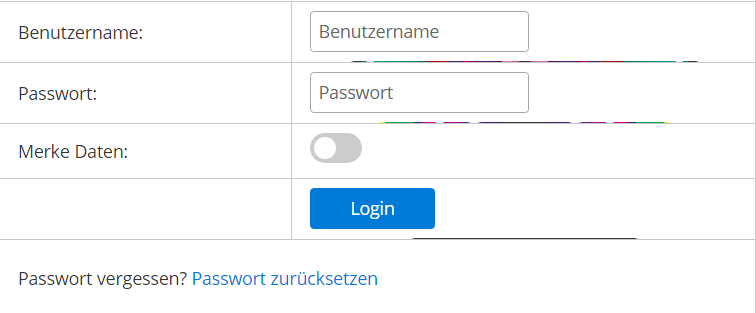
\includegraphics[width=\textwidth]{screenshots/allgemein/login.png}
  \caption{Nutzertabelle}
  \label{fig:boat1}
\end{center}
\end{figure}

\textbf{Hinweis:} Wenn Sie der Systemadministrator sind, und sich zum ersten Mal in diesem System anmelden, ist der Benutzername und das Passwort \textit{admin}. Es ist ratsam, dies möglichst schnell zu ändern. \\


\subsubsection{Passwort vergessen}
Wenn Sie Ihr Passwort vergessen haben, können Sie auf der Login-Seite auf Passwort vergessen klicken. Dadurch werden Sie auf eine Seite geleitet, wo Sie mithilfe Ihres Benutzernamens oder der Email Adresse, mit der Sie im System registriert sind, das Passwort zurücksetzen können. Dafür geben Sie einfach im entsprechenden Eingabefeld Ihre Daten ein, und klicken Sie auf Zurücksetzen. Dadurch wird ...? //TODO

\begin{figure}[h!]
\begin{center}
 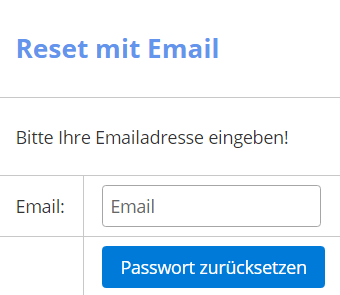
\includegraphics[width=\textwidth]{screenshots/allgemein/resetemail.png}
  \caption{Passwortzurücksetzung mit Email}
  \label{fig:boat1}
\end{center}
\end{figure}

\begin{figure}[h!]
\begin{center}
 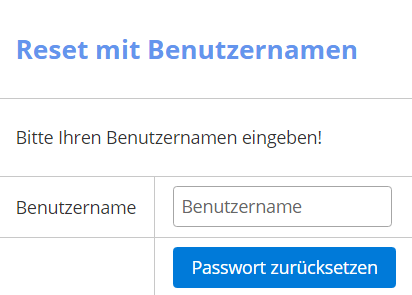
\includegraphics[width=\textwidth]{screenshots/allgemein/resetname.png}
  \caption{Passwortzurücksetzung mit Name}
  \label{fig:boat1}
\end{center}
\end{figure}



\subsection{Abmeldung}
Um sich abzumelden, klicken Sie in der Navigationsleiste am oberen Rand der Seite auf Logout. Sie werden dadurch zurück zu der Willkommensseite geleitet. \\


\subsection{Sprachauswahl}
Sie können zwischen Deutsch und Englisch als Anzeigesprachen wählen. Die Option dafür befindet sich unterhalb des Navigationsmenüs an der linken Seite. \\


\subsection{Navigationsleiste}
Es gibt zwei Navigationsleisten: Eine am oberen Rand, und eine am linken. \\


\subsubsection{Navigationsleiste links}
In der Navigationsleiste am linken Rand sehen Sie alle Aktionen, die Ihnen zur Verfügung stehen, sortiert nach den Rollen, die Sie haben. Sie können durch Klicken auf die Titel der Seiten auf die unterschiedlichen Seiten gehen. \\

\begin{figure}[h!]
\begin{center}
 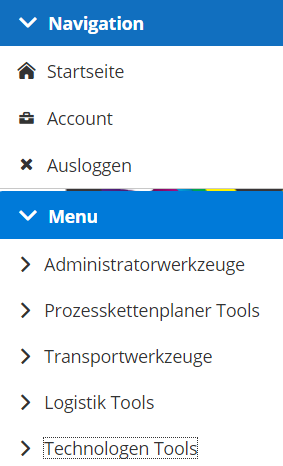
\includegraphics[width=\textwidth]{screenshots/allgemein/navigationlinks.png}
  \caption{Linke Navigationsleiste}
  \label{fig:boat1}
\end{center}
\end{figure}


\subsubsection{Navigationsleiste oben}
In der Navigationsleiste am oberen Rand können Sie durch Klicken auf Home zum Homescreen zurück //TODO.  \\


\begin{figure}[h!]
\begin{center}
 
\includegraphics[width=\textwidth]{screenshots/allgemein/willkommeneingeloggt.png}
  \caption{Nutzertabelle}
  \label{fig:boat1}
\end{center}
\end{figure}

Sie können ebenfalls unter Anlegen->New alle Gegenstände sehen, die Sie mit Ihren Rollen erstellen können. //TODO \\
Ebenfalls können Sie sich hier unter Logout abmelden. \\


\begin{figure}[h!]
\begin{center}
 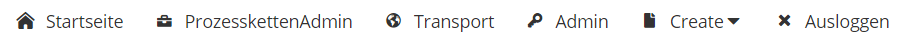
\includegraphics[width=\textwidth]{screenshots/allgemein/navigationoben.png}
  \caption{Obere Navigationsleiste}
  \label{fig:boat1}
\end{center}
\end{figure}

\begin{figure}[h!]
\begin{center}
 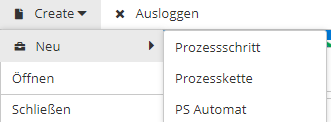
\includegraphics[width=\textwidth]{screenshots/allgemein/navigationcreate.png}
  \caption{Erstellen neuer Daten mit der oberen Navigationsleiste}
  \label{fig:boat1}
\end{center}
\end{figure}

%%%%%%%%%%%%%%%%%%%%%%%%%%%%%%%%%%%%%%%%%%%%%%%%%%%%%%%%%%%%%%%%%%%%%%%%

\newpage
\section{Farbige Zustände für Administratoren}
Hier finden Sie Anleitung für alle Aktionen, die ein Systemadministrator durchführen kann. 
%%%%%%%%%%
\subsection{Installation der Applikation}
\subsection{Vorbedingungen}
Vor dem Ausführen der Software muss überprüft werden, ob \$JAVA\_Home korrekt gesetzt wird.
Um dies zu prüfen, kann \textit{mvn -v} ausgeführt werden
Eine korrekte ausgabe ist:
\begin{verbatim}
Apache Maven 3.6.3 (NON-CANONICAL_2019-11-27T20:26:29Z_root)
Maven home: /opt/maven
Java version: 13.0.2, vendor: N/A, runtime: /usr/lib/jvm/java-13-openjdk
Default locale: de_DE, platform encoding: UTF-8
OS name: "linux", version: "5.5.6-arch1-1", arch: "amd64", family: "unix"
\end{verbatim}

Die Anwendung verwendet eine Integrationstest in Selenium and PhatomJs. Um diesen Testvorgang durchzuführen, muss der PhantomJS-Treiber installiert werden. Dieser Prozess muss ausgeführt werden, nach die Applikation Deployment Prozess. Der Normal Deployment Prozess der Applikation wegen diese Test wird nicht beeinträchtigt. In einigen Fällen können die gesuchten Elemente die Referenz in HTML ändern, infolgedessen nicht erfolgreich testen repräsentiert nicht unbedingt ein Problem an der Applikation.\\

Installation Methode:\\
durch brew
\begin{verbatim}
brew cast install phantomjs
\end{verbatim}
durch Dowloadwebseit:
\begin{verbatim}
https://phantomjs.org
\end{verbatim}
%%%%%%%%%%
\subsection{Benutzer}
Die Aktionen bezüglich der Benutzer des Systems können Sie unter dem Unterpunkt Nutzer Verwalten im Menü aufrufen. \\

Hier haben Sie eine Tabelle, die alle Benutzer anzeigt, die aktuell im System vorhanden sind. Die Benutzer werden für bessere Übersicht seitenweise angezeigt, mit den Knöpfen oberhalb und unterhalb der Tabelle können Sie durch diese Seiten navigieren.\\

\begin{figure}[h!]
\begin{center}
 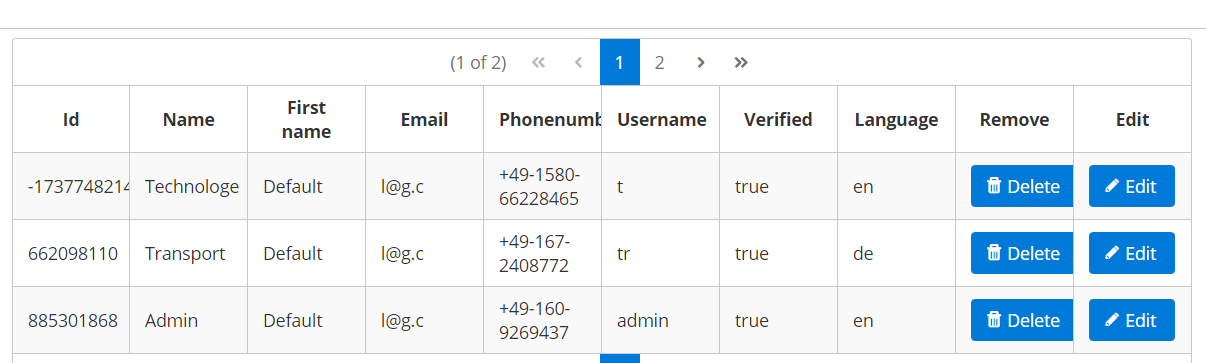
\includegraphics[width=\textwidth]{screenshots/admin/nutzertabelle.png}
  \caption{Nutzertabelle}
  \label{fig:boat1}
\end{center}
\end{figure}

 In dieser Tabelle können Sie durch drücken auf den Knopf Löschen den Benutzer der Zeile aus dem System entfernen.  \\
\begin{figure}[h!]
\begin{center}
 
\includegraphics[width=\textwidth]{screenshots/admin/nutzerloeschen.png}
  \caption{Nutzer erfolgreich gelöscht}
  \label{fig:boat2}
\end{center}
\end{figure}

Um Benutzer zu bearbeiten, drücken Sie auf den Knopf Bearbeiten, woraufhin die Daten des Users in das Formular oberhalb der Tabelle angezeigt werden, wo Sie Änderungen vornehmen können. \\
Bitte beachten Sie, in dem Feld Email nur Eingaben in der Form []@[].[] einzugeben, wobei die Endung länger als zwei Zeichen sein muss. Des weiteren dürfen für die Telefonnummer nur Zahlen eingegeben werden. Sollten Sie Fehler in den Eingaben machen, werden Ihnen die fehlerhaften Felder rot unterlegt. Die ID eines Benutzers können Sie nicht bearbeiten, da diese vom System verwaltet werden. \\
Mit Drücken auf Reset werden die bisher gespeicherten Daten wieder hergestellt. Mit Drücken auf Speichern können Sie Ihre Änderungen speichern. \\

//TODO Bild

Über der Tabelle befindet sich ein Formular, in dem Sie die Daten für einen neuen Benutzer eingeben können. Wenn sie alle Daten eingegeben haben, klicken Sie auf Speichern, um den Benutzer zu speichern. Die ID müssen Sie nicht selber eingeben, da sie vom System generiert wird. \\
Hier gelten die gleichen Beschränkungen wie oben für die Bearbeitung von Benutzern genannt. \\

\begin{figure}[h!]
\begin{center}
 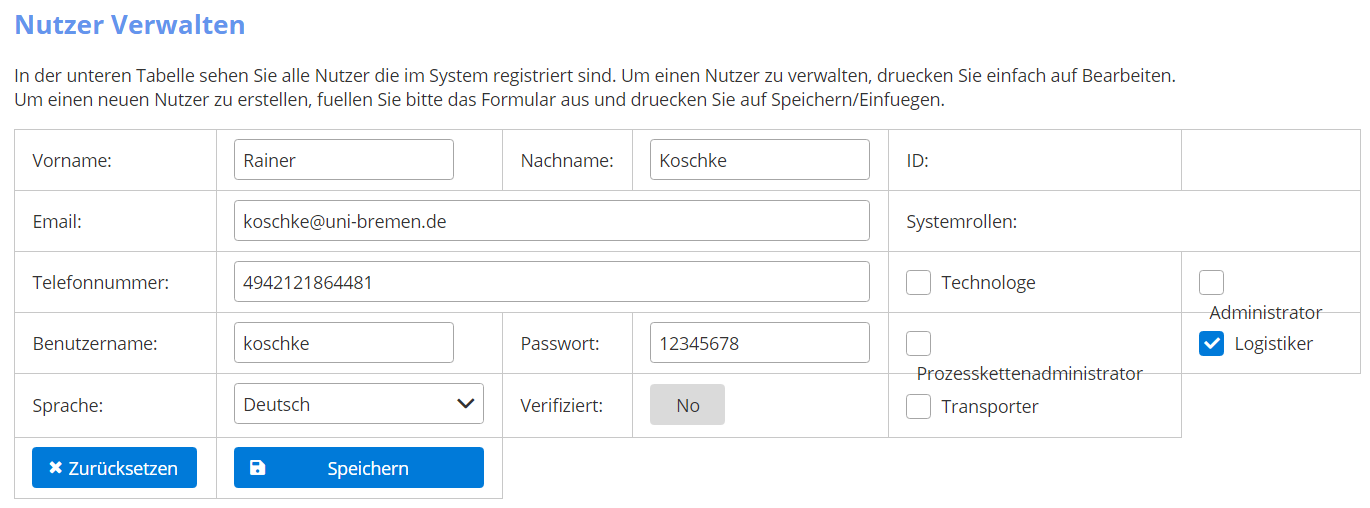
\includegraphics[width=\textwidth]{screenshots/admin/nutzerformularausgefuellt.png}
  \caption{Nutzerformular ausgefüllt}
  \label{fig:boat3}
\end{center}
\end{figure}

Bei erfolgreicher Erstellung eines Benutzer werden Sie eine Nachricht am rechten Rand des Fensters sehen, der neue Benutzer wird in der Tabelle erscheinen und eine Email bekommen. 
\begin{figure}[h!]
\begin{center}
 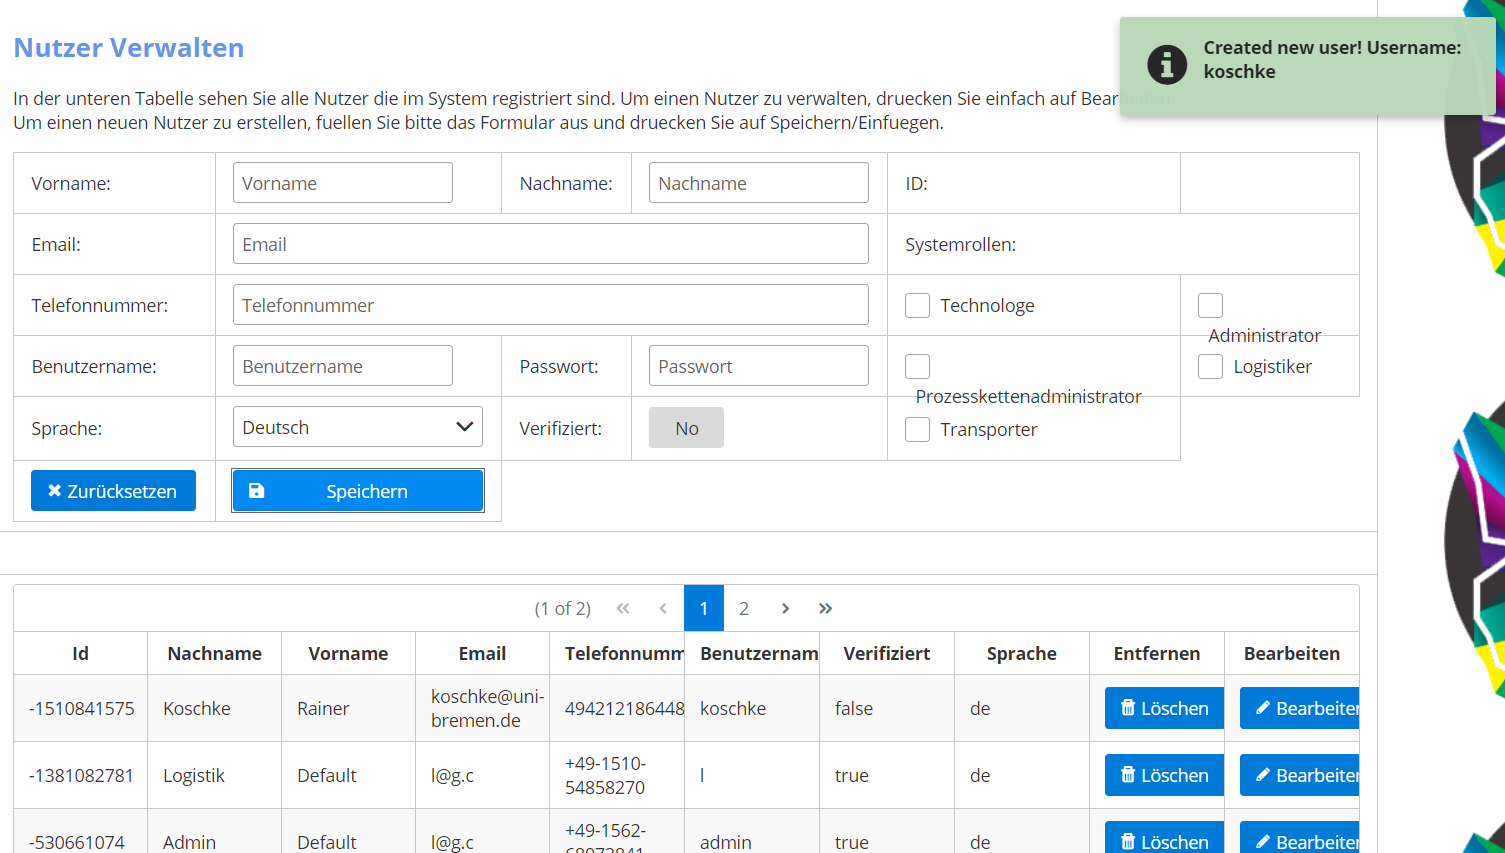
\includegraphics[width=\textwidth]{screenshots/admin/nutzererfolgreich.png}
  \caption{Nutzer erfolgreich gespeichert}
  \label{fig:boat1}
\end{center}
\end{figure}
Wenn sie die Daten im Formular zurücksetzen wollen, drücken Sie auf Reset. Dadurch werden keine Veränderungen an den vom System gespeicherten Daten vorgenommen. \\ 

\subsection{Experimentierstationen}
Die Aktionen bezüglich der Experimentierstationen können Sie unter dem Unterpunkt Experimentierstationen Verwalten im Menü aufrufen. \\
Auf der Seite sehen Sie eine Tabelle mit allen existierenden Experimentierstationen, sowie ein Formular für die Eingabe von Informationen einer Station. Die Tabelle zeigt die Stationen seitenweise an. Mithilfe der Knöpfe ober- und unterhalb der Tabelle können Sie durch die Seiten navigieren. \\

\begin{figure}[h!]
\begin{center}
 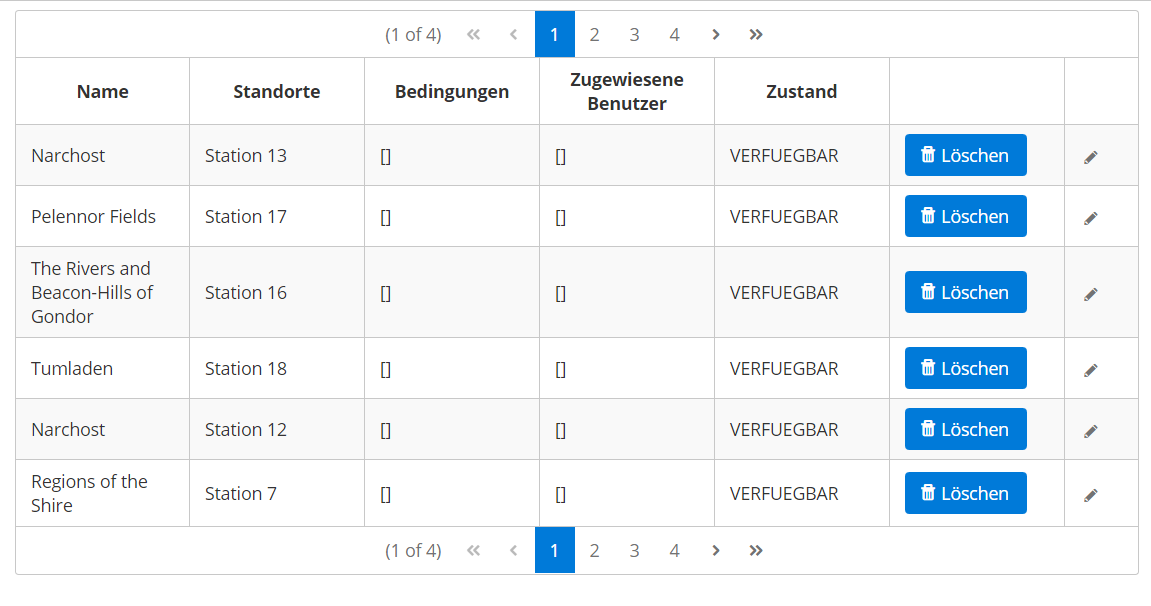
\includegraphics[width=\textwidth]{screenshots/admin/stationtabelle.png}
  \caption{Tabelle der Stationen}
  \label{fig:boat2}
\end{center}
\end{figure}

In dem Formular können Sie einen Namen eingeben, und einen Standort, die Prozessschrittparameter und die Benutzer, die an dieser Station arbeiten sollen, aussuchen. \\

\begin{figure}[h!]
\begin{center}
 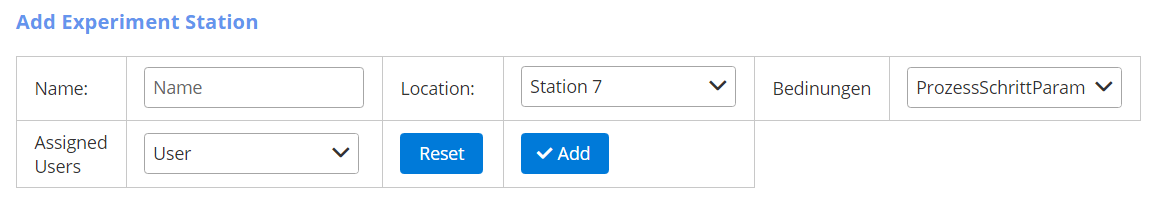
\includegraphics[width=\textwidth]{screenshots/admin/stationformular.png}
  \caption{Formular für Stationen}
  \label{fig:boat2}
\end{center}
\end{figure}

Für Benutzer, Parameter und Standort wählen Sie bitte die passenden Informationen aus der Liste, die Ihnen nach Klick auf das betreffende Feld angezeigt wird, aus. Bitte beachten Sie, dass alle Felder ausgefüllt sein müssen. \\

\begin{figure}[h!]
\begin{center}
 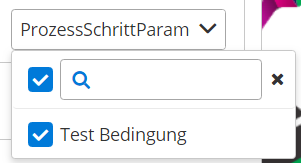
\includegraphics[width=\textwidth]{screenshots/admin/stationpsp.png}
  \caption{Prozessschrittparameter für Stationen}
  \label{fig:boat2}
\end{center}
\end{figure}

\begin{figure}[h!]
\begin{center}
 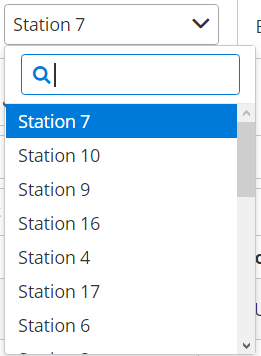
\includegraphics[width=\textwidth]{screenshots/admin/stationstandortliste.png}
  \caption{Station Standort List}
  \label{fig:boat2}
\end{center}
\end{figure}

\begin{figure}[h!]
\begin{center}
 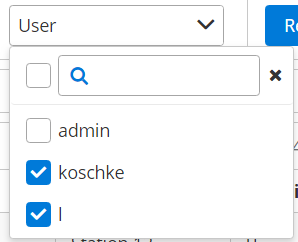
\includegraphics[width=\textwidth]{screenshots/admin/stationuser.png}
  \caption{Station Benutzer}
  \label{fig:boat2}
\end{center}
\end{figure}

Um die Station zu speichern, drücken Sie auf Erstellen, woraufhin Sie diese in der Tabelle sehen können. Um Ihre Eingaben zurückzusetzen, drücken Sie auf Zurücksetzen. \\


Wollen Sie eine existierende Station löschen, drücke Sie in der Tabellenzeile der Station auf Löschen. Die Station wird daraufhin aus der Tabelle entfernt. \\
Wenn Sie eine existierende Station bearbeiten wollen, drücken Sie in der Tabellenzeile auf den Stift. Daraufhin können Sie in die Zelle klicken, die Sie bearbeiten wollen, und dann die Informationen analog zur Eingabe im Formular auswählen. Nachdem Sie fertig sind mit der Bearbeitung der Station, klicken Sie bitte auf den Haken, der am Ende der Zeile statt des Stifts erschienen ist. Wenn Sie die Eingabe abbrechen wollen, drücken Sie auf das Kreuz. Auch hier müssen alle Felder ausgefüllt sein. \\

\begin{figure}[h!]
\begin{center}
 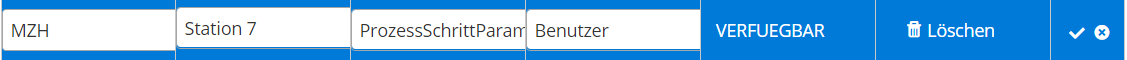
\includegraphics[width=\textwidth]{screenshots/admin/stationbearbeiten.png}
  \caption{Bearbeiten einer Station}
  \label{fig:boat2}
\end{center}
\end{figure}


%%%%%%%%%%

\subsection{Standorte}
Die Aktionen bezüglich der Standorte können Sie unter dem Unterpunkt Standort Verwalten im Menü aufrufen. \\
Auf dieser Seite sehen Sie eine Tabelle, in der alle existierenden Standorte angezeigt werden, und ein Feld, in dem Sie den Namen eines neuen Standorts eingeben können. \\

\begin{figure}[h!]
\begin{center}
 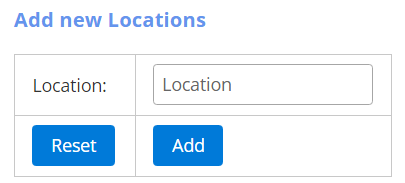
\includegraphics[width=\textwidth]{screenshots/admin/standortformular.png}
  \caption{Standort Formular}
  \label{fig:boat2}
\end{center}
\end{figure}

Um einen neuen Standort zu speichern, geben Sie einfach den Namen des Standorts in das Feld ein, und drücke Sie auf Erstellen. Nach erfolgreichem Speichern wird dieser der Tabelle hinzugefügt. \\

\begin{figure}[h!]
\begin{center}
 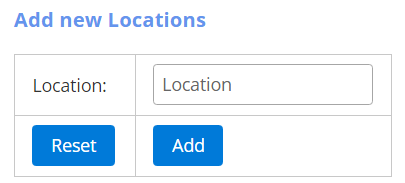
\includegraphics[width=\textwidth]{screenshots/admin/standortformular.png}
  \caption{Standortformular}
  \label{fig:boat2}
\end{center}
\end{figure}

Wenn Sie einen existierenden Standort löschen wollen, klicken Sie in der Tabellenzeile des Standorts auf Löschen. Der Standort verschwindet daraufhin aus der Tabelle. \\

Um einen existierenden Standort zu bearbeiten, klicken Sie in der entsprechenden Tabellenzeile auf das Stift Symbol. Daraufhin können Sie in die Zelle mit dem Namen klicken und diesen editieren. Wenn Sie fertig sind, klicken Sie auf den Haken, der am Ende der Zeile an der Stelle des Stifts erschienen ist. Wenn Sie den Vorgang abbrechen und auf den alten Namen zurücksetzen wollen, klicken Sie auf das Kreuz. \\

\begin{figure}[h!]
\begin{center}
 
\includegraphics[width=\textwidth]{screenshots/admin/standortbearbeiten.png}
  \caption{Standort Bearbeiten}
  \label{fig:boat2}
\end{center}
\end{figure}


%%%%%%%%%%
\subsection{Globale Einstellungen}
Unter dem Unterpunkt Globale Einstellungen können Sie die Zeiten von alten Aufträgen verwalten und ändern. \\
Auf der Seite können Sie eine Tabelle sehen, die alle Aufträge beinhaltet, die bereits vollständig bearbeitet wurden. Für jeden Auftrag können Sie die Zeiten für die Erstellung, den Start, die Beendung und die Archivierung sehen. \\
Wenn Sie die Zeiten eines Auftrags bearbeiten wollen, drücken Sie auf das Stift-Symbol in der entsprechenden Zeile. Daraufhin können Sie in die Zelle klicken, die Sie bearbeiten wollen, und eine neue Zeit eingeben. Zeiten werden wie folgt eingegeben: YYYY:MM:DDTHH:MM. 
Wollen Sie Ihre Änderungen speichern, klicken Sie auf den Haken, der anstelle des Stifts erschienen ist. Wollen Sie Ihre ungespeicherten Änderungen zurücksetzen, klicken Sie auf das Kreuz neben dem Haken. \\
Bitte beachten Sie, dass für jeden Auftrag alle vier Zeiten angegeben sein müssen, und Sie keine Zeiten löschen können. \\

%%%%%%%%%%
\subsection{Backup der Systemdaten}
Unter dem Unterpunkt Backup und Wiederherstellen können Sie die aktuelle Datenbank mit all ihrer Daten exportieren, oder neue Daten aus einer existierenden Datenbank importieren. \\

Um ein Backup der Daten zu erstellen, müssen Sie nur auf Backup Erstellen klicken. Daraufhin wird ein Backup automatisch erstellt. //TODO \\

Wollen Sie Daten aus einer Datei einlesen, klicken Sie auf Choose. Daraufhin öffnet sich ein Fenster, in dem Sie aus Ihrem Dateisystem die Datei auswählen können. Wenn Sie eine Datei ausgewählt haben, drücken Sie auf Öffnen, woraufhin die Datei hochgeladen wird. Mit einem Klick auf Submit werden die Daten aus der Datei in die Datenbank integriert. Bitte beachten Sie, dass  Sie eine SQL Datei auswählen müssen. \\ 

\subsection{Fehler und Ursachen}
\begin{longtable}[c]{|p{5cm}|p{10cm}|}
\hline
\multicolumn{1}{|c|}{\textbf{Hinweis}}                          & \multicolumn{1}{c|}{\textbf{Ursache}}                                                                                                                                                                                                               \\ \hline
\endhead
Couldn't update user! ID..  & Der Benutzer wurde nicht in der Datenbank gefunden. Bitte fügen Sie einen neuen Benutzer hinzu.\\ \hline
Couldn't delete user! ID .. & Der Benutzer wurde nicht in der Datenbank gefunden. \\ \hline
Couldn't update experimentierstatioN! ID .. & Die Station wurde nicht in der Datenbank gefunden. Bitte fügen Sie die Station neu hinzu. \\ \hline
Error adding experimenting station, station already exists! Name: ..  & Es existiert bereits eine Station mit dem Namen, unter dem Sie die neue speichern wollen. \\ \hline
Couldn't add experimenting station! Name .. & Ein interner Systemfehler ist aufgetreten. Bitte versuchen Sie, die Station unter einem anderen Namen zu speichern. Wenn dies nicht funktioniert, kontaktieren Sie das Entwicklerteam. \\ \hline
Couldn't delete experimenting station! ID .. & Die Station wurde nicht in der Datenbank gefunden. \\ \hline
Couldn't update job! ID .. & Die Station wurde nicht in der Datenbank gefunden. Bitte fügen Sie die Station neu hinzu. \\ \hline
Couldn't import data! & Es ist ein Fehler beim Einlesen der Datei, die Sie ausgewählt haben. Bitte stellen Sie sicher, dass die Datei das korrekte Format hat. \\ \hline
Couldn't backup database! & Es ist ein interner Fehler aufgetreten. Bitte kontaktieren Sie das Entwicklerteam. \\ \hline
Standort with name .. already exists! & Es existiert bereits ein Standort mit dem Namen, unter dem Sie die neue speichern wollen. \\ \hline
Couldn't add new location with name .. & Es ist ein interner Systemfehler aufgetreten. Bitte versuchen Sie, den Standort unter einem Namen zu speichern. Wenn das nicht funktioniert, kontaktieren Sie das Entwicklerteam. \\ \hline
Couldn't update location object with id .. & Der Standort wurde nicht in der Datenbank gefunden. Bitte fügen Sie den Standort neu hinzu. \\ \hline
Failed to remove location with id .. & Der Standort wurde nicht in der Datenbank gefunden. Wenn Sie den Standort aus der Datenbank entfernen wollten, müssen Sie also nichts weiter tun. \\ \hline
\end{longtable}
%%%%%%%%%%%%%%%%%%%%%%%%%%%%%%%%%%%%%%%%%%%%%%%%%%%%%%%%%%%%%%%%%%%%%%%%

\newpage
\section{Farbige Zustände für andere Mitarbeiter}
\subsection{Prozesskettenadministrator}

Hier finden Sie Anleitungen für alle Aktionen, die ein Prozesskettenadministrator ausführen kann.
%%%%%%%%%%
\subsubsection{Prozessschritte}

Im Menü-Unterpunkt Prozessschritt haben Sie eine Übersicht über alle Prozessschritte, die aktuell im System existieren, können diese bearbeiten und löschen, sowie neue hinzufügen. Prozessschritte werden seitenweise angezeigt, Sie können durch die Seiten mithilfe der Navigatoren ober- und unterhalb der Tabelle navigieren. Bitte beachten Sie, dass Sie nur Schritte bearbeiten und löschen können, die noch nicht gestartet wurden. \\

Prozessschritte sind die Prozessschritte, die zu Aufträgen, instanziierten Prozesskettenvorlagen, gehören. \\

Wenn Sie einen neuen Prozessschritt erstellen wollen, geben Sie bitte im Formular am Anfang der Seite alle Informationen für diesen ein. Dazu gehört, dass Sie eine existierende Vorlage auswählen, einen Namen eingeben, und Attribute //TODO. Bitte beachten Sie, dass Sie in allen Feldern Eingaben machen müssen. Um diesen Schritt zu speichern, drücken Sie auf Speichern. Nach der erfolgreichen Speicherung wird dieser in der Tabelle zu sehen sein. Um das Formular zurückzusetzen, drücken Sie auf Zurücksetzen; dadurch entstehen keine Änderungen am Datensatz im System. \\

\begin{figure}[h!]
\begin{center}
 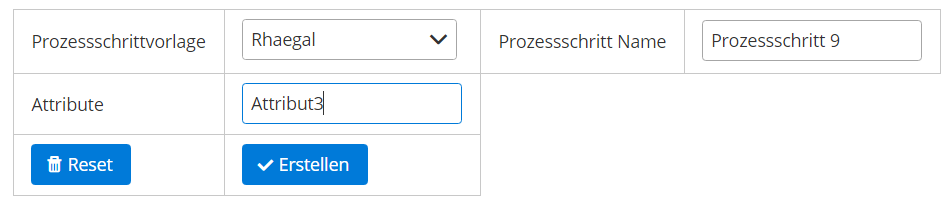
\includegraphics[width=\textwidth]{screenshots/pk/01prozessschrittformular.png}
  \caption{Das Formular für neue Prozessschritte}
  \label{fig:boat2}
\end{center}
\end{figure}

In der Tabelle der existierenden Prozessschritte können Sie mit Klicken auf Anzeigen in den Spalten Eingabeträger, Ausgabeträger, Prozessschritt-Parameter sowie Prozessschritt-Log Details zu den jeweiligen Eigenschaften eines bestimmten Prozessschrittes einsehen. \\

Wenn Sie einen existierenden Prozessschritt bearbeiten wollen, drücken Sie in der Zeile, in der der gewünschte Schritt in der Tabelle steht, auf das Stift-Symbol. Danach können Sie in die Zelle, die Sie bearbeiten wollen, klicken, und die Änderungen vornehmen. Bitte beachten Sie, dass Sie den Status und den Log nicht bearbeiten können. Wenn Sie fertig mit Ihren Änderungen sind, drücken Sie auf den Haken, der an der Stelle des Stifts erschienen ist. Wenn Sie ungespeicherte Änderungen zurücksetzen wollen, drücken Sie auf das Kreuz; dadurch werden die Daten für den Prozessschritt auf den aktuellen Stand in der Datenbank gesetzt. \\


Wollen Sie einen Prozessschritt löschen, drücken Sie auf das Löschen Symbol in der Zeile des Schrittes, den Sie löschen wollen. \\

//TODO Logs, Parameter anzeigen
%%%%%%%%%%
\subsubsection{Prozessschritt Vorlage}

Im Menü-Unterpunkt Prozessschritt Vorlage haben Sie eine Übersicht über alle in der Datenbank existierenden Prozessschritt Vorlagen, können diese bearbeiten und Löschen, sowie neue hinzufügen. \\

Prozessschrittvorlagen können Sie im Menüunterpunkt Prozesskettenvorlagen benutzen, um die zu einer Kettenvorlage gehörigen Schritte zu definieren. \\

Um eine neue Vorlage zu speichern, geben Sie bitte in das Formular alle Informationen ein. Dafür müssen Sie aus den bestehenden Parametern alle, die hier zutreffen, die richtige Zustandsautomat Vorlage, die möglichen Trägerarten für Ein- und Ausgabe, und die Experimentierstationen, an denen dieser Schritt ausgeführt werden kann, auswählen, sowie die Dauer, die dieser Schritt vorraussichtlich haben wird und den Namen der neuen Vorlage eingeben. Zusätzlich müssen Sie auswählen, ob der Schritt Urformend sein wird, das heißt, ob durch die Ausführung des Schrittes neue Proben entstehen. Wenn der Prozessschritt urformend sein soll, geben Sie bitte im Feld daneben die Anzahl an Proben an, die erstellt werden, sowie die Proben-ID für die Proben, die erstellt werden. Bitte beachten Sie, dass Sie für alle Felder Angaben machen müssen. Die Dauer muss von der Form xx:xx sein, und darf nicht 23:59 überschreiten. Um die neue Vorlage zu speichern, drücken Sie auf Erstellen. Danach wird die neue Vorlage in der Tabelle angezeigt. Wenn Sie Ihre Eingaben löschen wollen, drücken Sie auf Zurücksetzen, dadurch werden keine Veränderungen an den Daten in der Datenbank vorgenommen. \\

\begin{figure}[h!]
\begin{center}
 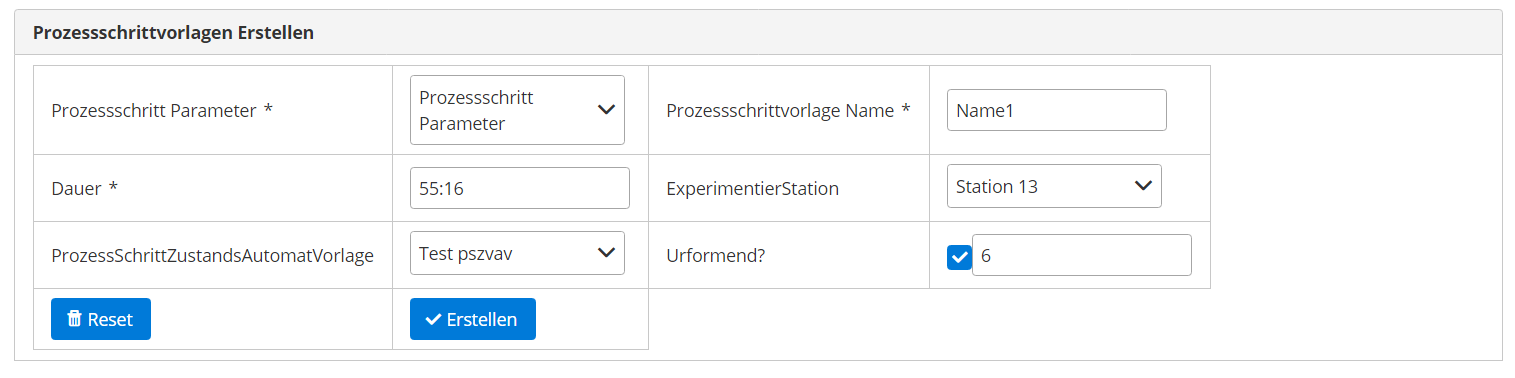
\includegraphics[width=\textwidth]{screenshots/pk/prozessschrittvorlageformular.png}
  \caption{Das Formular für eine neue Prozessschrittvorlage}
  \label{fig:boat2}
\end{center}
\end{figure}

\begin{figure}[h!]
\begin{center}
 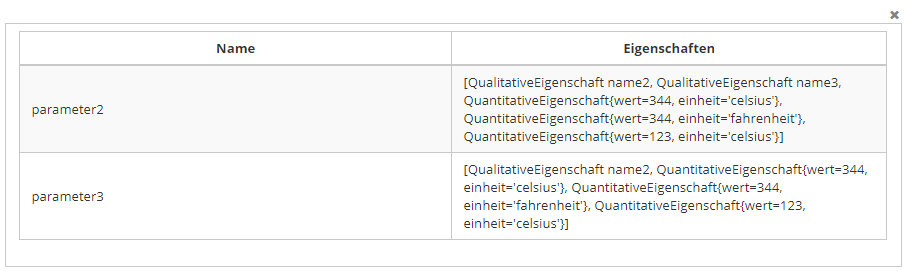
\includegraphics[width=\textwidth]{screenshots/pk/prozessschrittvorlageparameter.png}
  \caption{Auswählen von Parametern für Prozessschritt Vorlagen}
  \label{fig:boat2}
\end{center}
\end{figure}

In der Tabelle der existierenden Prozessschritt-Vorlagen können Sie die Eingabe und Ausgabe Träger sowie die Prozessschritt-Parameter, die zu einer bestimmten Vorlage gehören, mit Klicken auf Anzeigen in den entsprechenden Spalten der zugehörigen Zeile einsehen. \\

Für die Bearbeitung von einer Vorlage drücken Sie in der entsprechenden Tabellenzeile auf das Stift-Symbol. Danach können Sie in die Zellen klicken, die Sie bearbeiten wollen, und die entsprechenden Änderungen machen. Um Ihre Änderungen zu speichern, drücken Sie auf den Haken, der an der Stelle des Stifts erschienen ist. Durch Drücken auf das Kreuz können Sie Ihre Änderungen zurücksetzen auf die Daten, die in der Datenbank gespeichert sind. \\

\begin{figure}[h!]
\begin{center}
 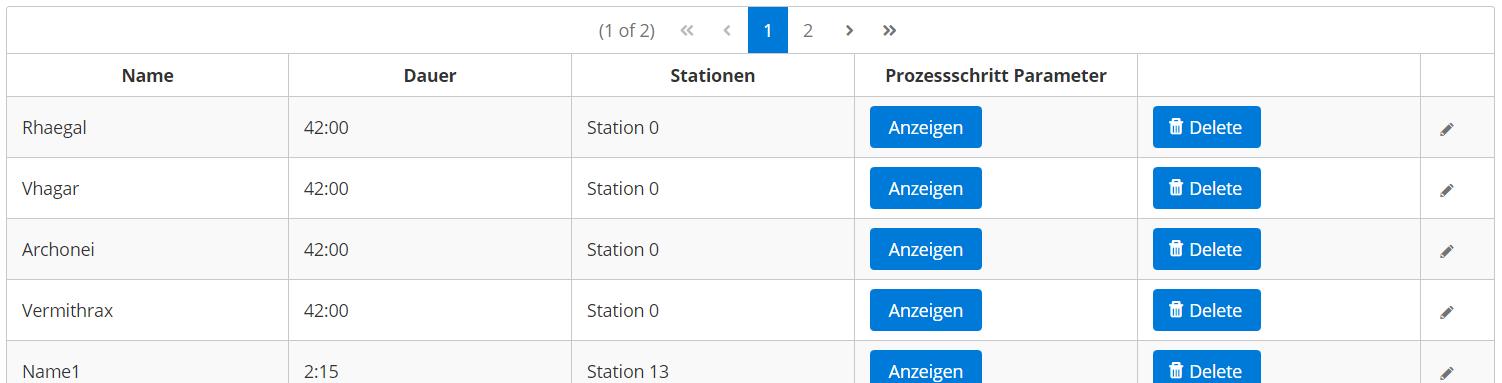
\includegraphics[width=\textwidth]{screenshots/pk/prozessschrittvorlagetabelle.png}
  \caption{Die Tabelle für die Prozessschritt Vorlagen}
  \label{fig:boat2}
\end{center}
\end{figure}


Wollen Sie eine Vorlage löschen, drücken Sie in der entsprechenden Tabellenzeile auf Löschen. \\


%%%%%%%%%%
\subsubsection{Prozessschritt Zustandsautomat}

Im Menü-Unterpunkt Prozessschrittzustandsautomatvorlagen Verwaltung haben Sie eine Übersicht über alle in der Datenbank existierenden Prozessschrittzustandsautomatvorlagen, können diese bearbeiten und löschen, sowie neue hinzufügen. \\

Prozessschritt Zustandsautomaten können Sie im Menüunterpunkt Prozessschritt Vorlage benutzen, um einen Zustandsautomaten für eine Prozessschrittvorlage festzulegen. \\

In der Tabelle der aktuell in der Datenbank gespeicherten Vorlagen können Sie mit den Navigatoren ober- und unterhalb der Tabelle zwischen den Seiten navigieren, alle Felder durch das Suchfeld \"Search all fields\" nach Schlagwörtern durchsuchen, ebenso sowie die Spalten Name und Zustandsreihenfolge durch die Suchfelder in den jeweiligen Spalten. \\
Durch die Felder in der ganz linken Spalte der Tabelle können Sie Vorlagen auswählen, um //TODO \\

\begin{figure}[h!]
\begin{center}
 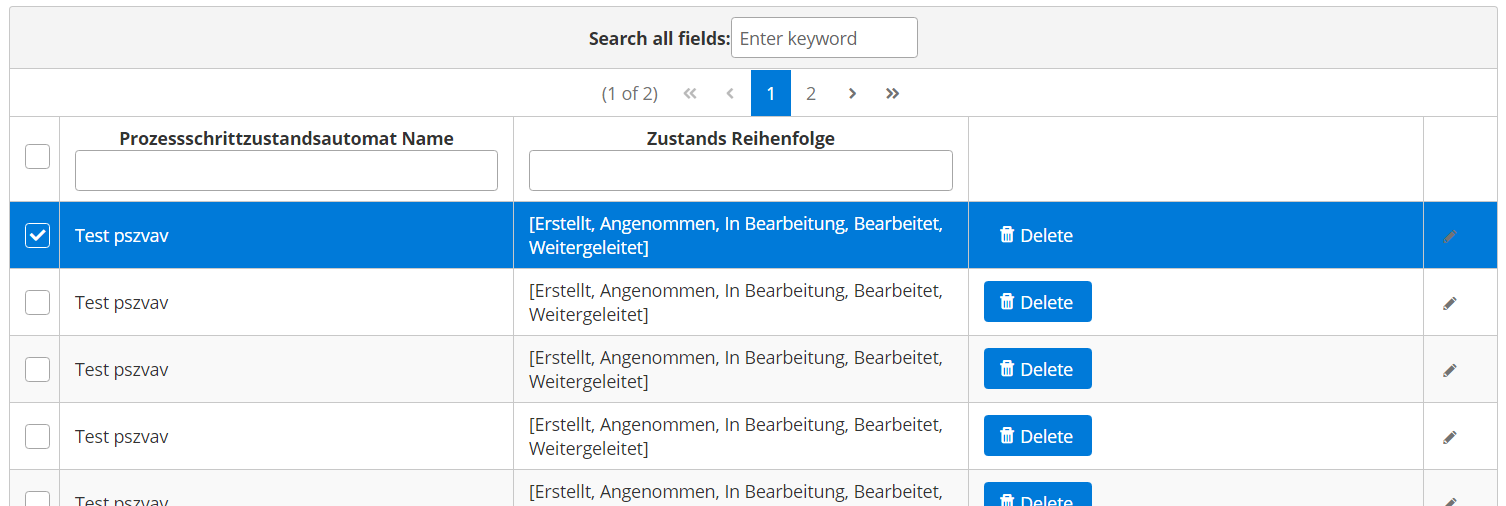
\includegraphics[width=\textwidth]{screenshots/pk/zustandsautomattabelle.png}
  \caption{Tabelle für die Zustandsautomat Vorlagen}
  \label{fig:boat2}
\end{center}
\end{figure}

Wollen Sie einen neuen Zustandsautomat erstellen, benutzen Sie das Formular am Anfang der Seite. Dort können Sie im Eingabefeld \"Zustaende einfuegen\" den Namen eines neuen Zustands eingeben, und Ihn durch Klicken auf Einfuegen in die Liste an Zuständen in der Anzeige "Zustandsautomat Erstellen" einfügen. Dort wird er auf der linken Seite am Ende der dort bereits stehenden Liste erscheinen. In dieser Anzeige können Sie die Zustände mit den Rechts- und Linkspfeilen zwischen dem rechten und linken Feld hin-und herschieben, wo sie jeweils am Ende der List stehen werden. Die doppelten Pfeile bewegen alle Zustände von einer Seite zu der anderen und behalten dabei die Reihenfolge, in der Sie in Ihrem ursprünglichen Feld standen. Sie müssen die Zustände in der richtigen Reihenfolge auf der rechten Seite sortieren. In der unteren Zeile können Sie einen Namen für Ihre neuen Zustandsautomatenvorlage eingeben. Bitte beachten Sie, dass jede Vorlage einen Zustand Erstellt enthalten muss, der am Anfang des Zustandsautomat steht. 
Nachdem Sie die Zustände auf der rechten Seite richtig stehen haben und einen Namen haben, können Sie auf Erstellen drücken, um die Vorlage zu erstellen, und in die Tabelle der existierenden Vorlagen einzufügen. Durch Drücken auf Zurücksetzen können Sie im Formular Ihre Änderungen löschen, wodurch keine Änderungen an den Daten in der Datenbank entstehen. \\

\begin{figure}[h!]
\begin{center}
 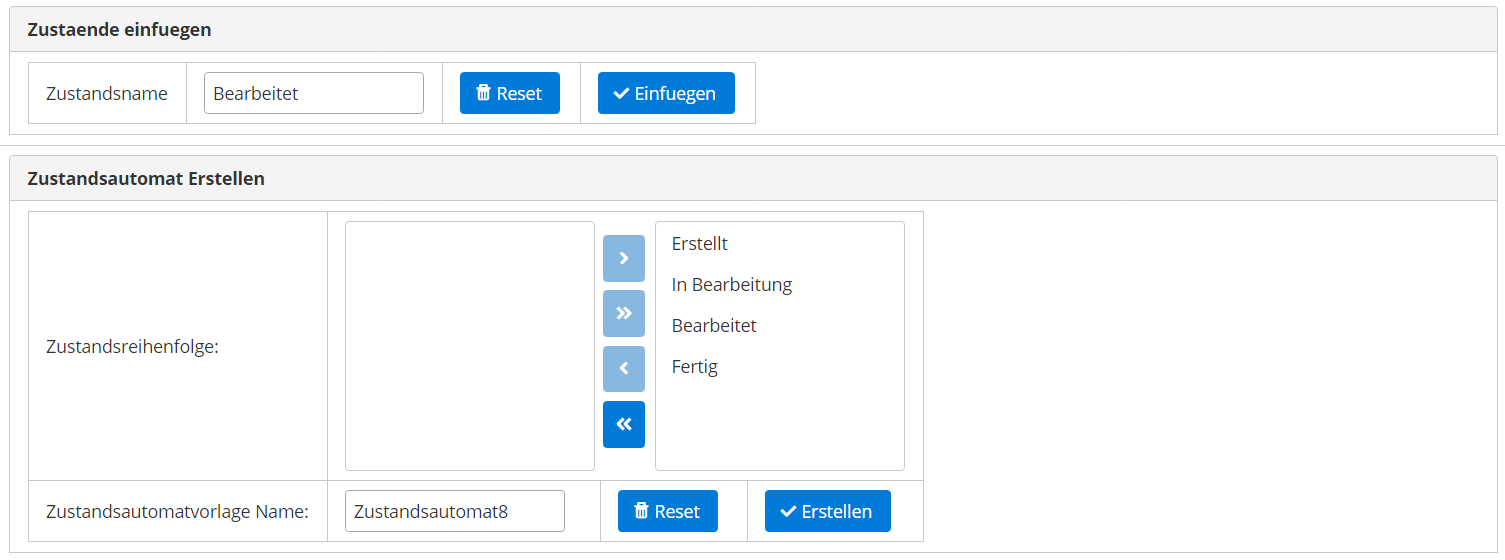
\includegraphics[width=\textwidth]{screenshots/pk/zustandsautomatformular.png}
  \caption{Formular für neue Zustandsautomat Vorlagen}
  \label{fig:boat2}
\end{center}
\end{figure}


Wenn Sie eine Zustandsautomatvorlage löschen wollen, drücken Sie auf Löschen in der entsprechenden Tabellenzeile. Dadurch wird die Vorlage aus der Datenbank entfernt, und kann nicht wieder hergestellt werden. \\


Um eine Vorlage zu bearbeiten, drücken Sie in der Tabellenzeile der gewünschten Vorlage auf das Stift-Symbol. Danach können Sie die gewünschten Änderungen eingeben, wobei das Bewegen der Zustände mit den Pfeiltasten zwischen den beiden Feldern ermöglicht wird. Die richtige Zustandsreihenfolge soll am Ende auf der rechten Seite stehen. Nachdem Sie alle gewünschten Änderungen gemacht haben, drücken Sie auf den Haken, der an Stelle des Stifts erschienen ist, wodurch diese gespeichert werden. Wenn Sie die Änderungen verwerfen und die Daten auf die in der Datenbank gespeicherten zurücksetzen wollen, drücken Sie auf das Kreuz. \\

\begin{figure}[h!]
\begin{center}
 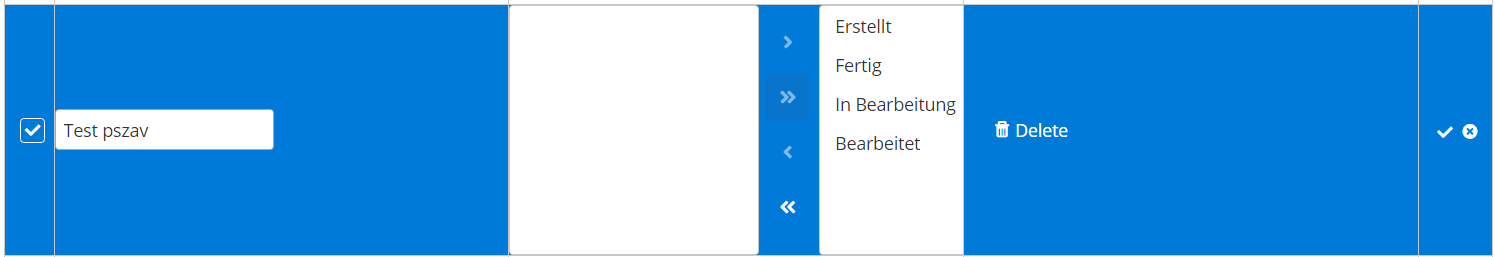
\includegraphics[width=\textwidth]{screenshots/pk/zustandsautomatbearbeiten.png}
  \caption{Bearbeiten einer Zustandsautomat Vorlage}
  \label{fig:boat2}
\end{center}
\end{figure}

%%%%%%%%%%
\subsubsection{Prozessschritt Parameter}

Im Menü-Unterpunkt Prozessparameter Verwaltung haben Sie eine Übersicht über die in der Datenbank gespeicherten Prozessparameter, können diese löschen und bearbeiten sowie neue erstellen. \\

Die Prozessschritt-Parameter können Sie im Menü-Unterpunkt Prozessschritt Vorlage Prozessschrittvorlagen hinzufügen. \\

In der Tabelle haben Sie eine Übersicht über alle existierenden Prozessparameter. Sie können jeweils durch Klicken auf Anzeigen Details zu den Qualitativen und Quantitativen Eigenschaften, die ein Parameter hat, einsehen. Mithilfe der Pfeiltasten können Sie zwischen den Seiten der Tabellen navigieren. \\


\begin{figure}[h!]
\begin{center}
 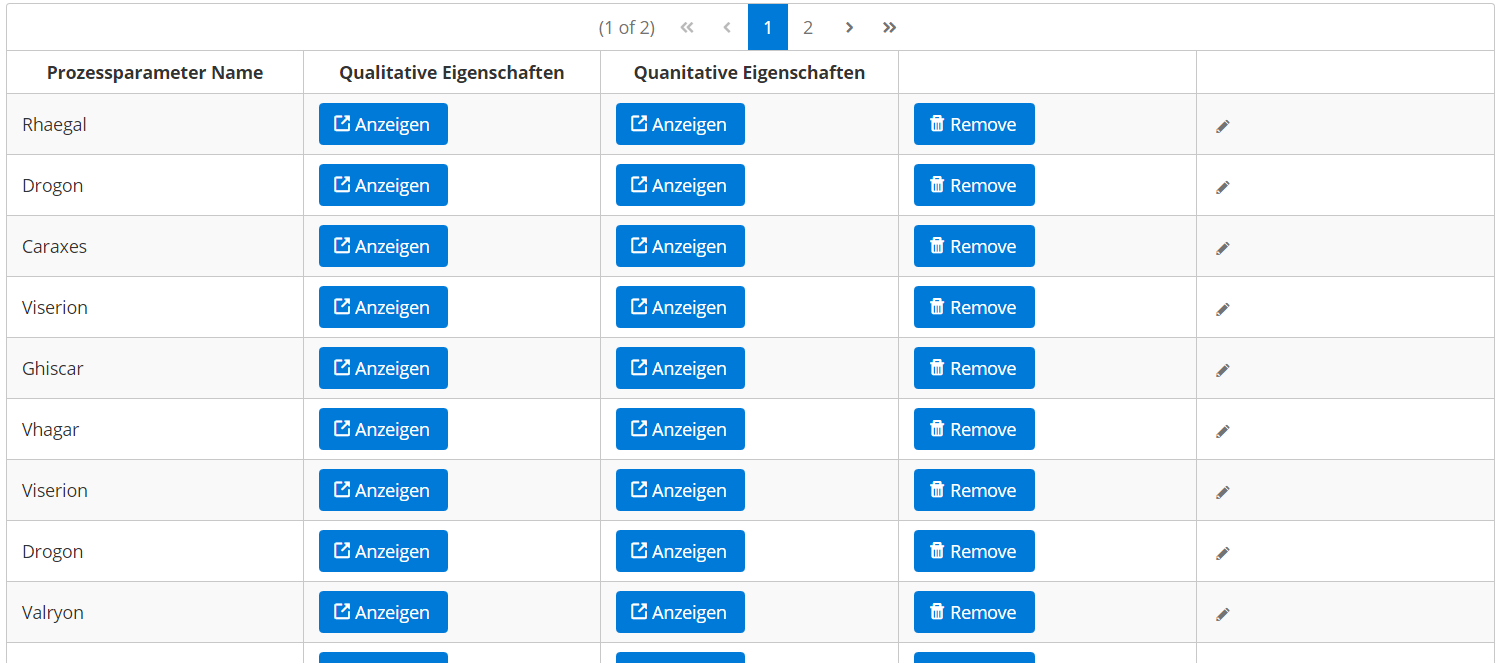
\includegraphics[width=\textwidth]{screenshots/pk/parametertabelle.png}
  \caption{Tabelle der Prozessparameter}
  \label{fig:boat2}
\end{center}
\end{figure}


Wollen Sie einen neuen Parameter erstellen, geben Sie im Formular alle notwendigen Informationen an: geben Sie einen Namen ein, und wählen Sie aus den existierenden Qualtitativen und Quantitiativen Eigenschaften die zugehörigen aus. Bitte beachten Sie, dass Sie für alle Felder angaben machen müssen. Wenn Sie das Formular ausgefüllt haben, können Sie diesen mit Einfuegen speichern. Durch drücken auf Zuruecksetzen können Sie die Felder im Formular löschen; hierdurch entstehen keine Änderungen an den Daten in der Datenbank. \\

\begin{figure}[h!]
\begin{center}
 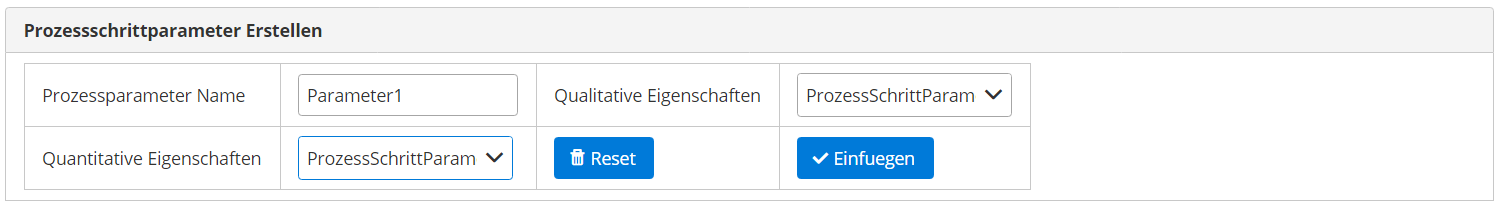
\includegraphics[width=\textwidth]{screenshots/pk/parameterformular.png}
  \caption{Formular für Erstellung eines Parameters}
  \label{fig:boat2}
\end{center}
\end{figure}


\begin{figure}[h!]
\begin{center}
 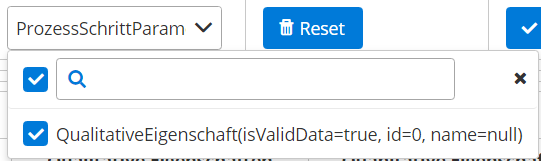
\includegraphics[width=\textwidth]{screenshots/pk/parameterquanti.png}
  \caption{Liste der quantitativen Eigenschaften für die Erstellung eines Parameters}
  \label{fig:boat2}
\end{center}
\end{figure}

\begin{figure}[h!]
\begin{center}
 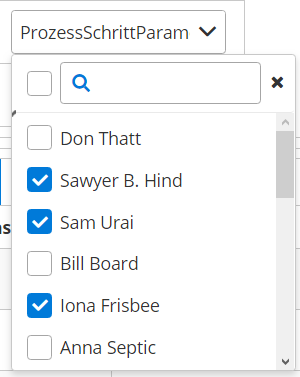
\includegraphics[width=\textwidth]{screenshots/pk/parameterliste.png}
  \caption{Liste der qualitativen Eigenschaften für die Erstellung eines Parameters}
  \label{fig:boat2}
\end{center}
\end{figure}

Um einen existierenden Parameter zu löschen, drücken Sie in der zugehörigen Tabellenzeile auf Loeschen. \\

Zum Bearbeiten eines Parameters, drücken Sie auf das Stift-Symbol in der zugehörigen Tabellenzeile. Danach können Sie in der Zeile die Zelle auswählen, die Sie bearbeiten wollen, und Ihre Änderungen vornehmen. Bitte beachten Sie, dass alle Zellen weiterhin Informationen enthalten müssen. Um Ihre Änderungen zu speichern, drücken Sie auf den Haken, der anstelle des Stift-Symbols erschienen ist; um sie zu verwerfen und die Daten auf die in der Datenbank gespeicherten zurückzusetzen, wählen Sie das Kreuz. \\

\begin{figure}[h!]
\begin{center}
 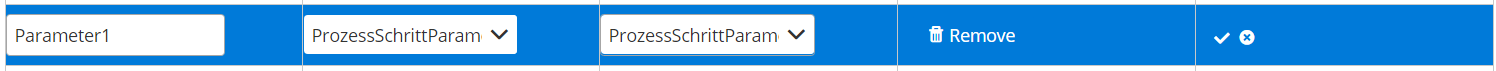
\includegraphics[width=\textwidth]{screenshots/pk/parameterbearbeiten.png}
  \caption{Bearbeiten eines Parameters}
  \label{fig:boat2}
\end{center}
\end{figure}


%%%%%%%%%%
\subsubsection{Prozessketten Vorlagen}

Im Menü-Unterpunkt Prozesskettenvorlagen Verwaltung haben Sie eine Übersicht über existierende Prozesskettenvorlagen, können diese löschen und bearbeiten sowie neue hinzufügen. \\

Die Prozesskettenvorlagen können Sie im Menü-Unterpunkt Auftraege zu Aufträgen instanziieren. \\

Benutzen Sie das Formular am Anfang der Seite, um eine neue Vorlage anzulegen. Hier wählen Sie aus den existierenden Prozessschritt-Vorlagen diejenigen aus, aus denen diese Vorlage bestehen soll, aus. Die existierenden stehen in dem linken Feld, und können durch Mausklick ausgewählt und mit den Pfeiltasten in der Mitte in das rechte Feld verschoben werden. Im rechten Feld sollten Sie am Ende alle Prozessschritt-Vorlagen, die verwendet werden sollen, in der Reihenfolge, in der Sie bearbeitet werden sollen, stehen. Im Eingabefeld darunter können Sie einen Namen für die neue Vorlage auswählen. Wenn Sie alle Angaben gemacht haben, können Sie die neue Vorlage mit Klick auf Erstellen speichern. Mit Zurücksetzen können Sie alle Angaben im Formular zurücksetzen, wodurch keine Änderungen an den in der Datenbank gespeicherten Daten gemacht werden. \\

In der Tabelle können Sie mit den Pfeiltasten ober-und unterhalb der Tabelle zwischen den Seiten navigieren. Die einzelnen Prozessschritt-Vorlagen, die zu den Prozessketten Vorlagen in der Tabelle gehören, können Sie mit Klick auf Anzeigen in der entsprechenden Tabellenzeile einsehen. \\

Um eine Prozesskettenvorlage zu löschen, können Sie in der entsprechenden Tabellenzeile, in der die gewünschte Vorlage zu sehen ist, auf Löschen klicken. Dadurch werden die Daten dieser Vorlage aus der Datenbank entfernt; die Daten der assoziierten Prozessschritt-Vorlagen bleiben jedoch unabhängig bestehen. \\

Wollen Sie eine existierende Prozesskettenvorlage bearbeiten, können Sie in der entsprechenden Tabellenzeile auf das Stift-Symbol drücken, und danach die entsprechenden Änderungen machen. Die zugehörigen Prozessschritt-Vorlagen können Sie zwischen den beiden Feldern mit den Pfeiltasten bewegen. Die Prozessschritt-Vorlagen, die am Ende in der Prozesskettenvorlage enthalten sein sollen, müssen auf der rechten Seite in der richtigen Reihenfolge (vom ersten zum letzten) stehen. Zu Beginn der Bearbeitung stehen im linken Feld alle in der Datenbank enthaltenen Prozessschritt-Vorlagen. Um Ihre Änderungen zu speichern, drücken Sie auf den Haken, der an der Stelle des Stift-Symbols erschienen ist; um sie zu verwerfen, drücken Sie auf das Kreuz. \\

%%%%%%%%%%
\subsubsection{Aufträge}

Im Menü-Unterpunkt Auftragsverwaltung haben Sie eine Übersicht über alle Aufträge, also instanziierte Prozesskettenvorlagen, die aktuell in der Datenbank existieren, können diese löschen und bearbeiten, sowie neue erstellen. \\

Neue Aufträge können Sie entweder aus Prozesskettenvorlagen instanziieren, oder aus Prozessschritt-Vorlagen zusammensetzen. \\

Für die Instanziierung aus Prozesskettenvorlagen wählen Sie im Formular am Anfang der Seite die entsprechende Vorlage aus, und geben Sie eine Priorität und einen Namen an. \\

Das zweite Formular auf der Seite können Sie für die Erstellung aus Prozessschrittvorlagen verwenden. Dort wählen Sie aus allen existierenden Vorlagen, die auf der linken Seite stehen, die aus, die Sie verwenden wollen, und bewegen Sie mit den Pfeiltasten in der Mitte in das linke Feld. Dort sollten die Schritte in der richtigen Reihenfolge von Start zu Ende stehen. Unterhalb dieser Felder können Sie einen Namen für den Auftrag eingeben, und eine Priorität auswählen. \\

In beiden Formularen können Sie, nachdem Sie alle Angaben gemacht haben, mit Klicken auf Erstellen den Auftrag erstellen. Durch Klicken auf Zurücksetzen können Sie die Angaben im Formular löschen, wodurch keine Änderungen an den Daten in der Datenbank entstehen. \\

In der Tabelle am Ende der Tabelle können Sie die existierenden Aufträge ansehen. Für eine Übersicht über die Prozessschritte eines bestimmten Auftrag können Sie in der zugehörigen Tabellenzeile auf Anzeigen in der Prozessschritt-Spalte klicken. \\

Wollen Sie einen Auftrag löschen, klicken Sie in der zugehörigen Tabellenzeile auf Löschen. \\ 
//TODO dies geht nur, solange der Auftrag nicht freigegeben wurde. 

Um einen Auftrag freizugeben, wodurch dieser an die Logistiker weitergegeben wird, klicken Sie in der zugehörigen Tabellenzeile auf Freigeben. \\

Wenn ein Auftrag bereits von einem Logistiker gestartet wurde, können Sie diesen mit Klicken auf Abbrechen, abbrechen. Alle Proben dieses Auftrags werden dadurch sofort ins Lager zurückgebracht. \\

%%%%%%%%%%
\subsubsection{Qualitative/Quantitative Eigenschaften}

Im Menü-Unterpunkt Qualitative/Quantitative Eigenschaften haben Sie eine Übersicht über die in der Datenbank gespeicherten qualitativen und quantitativen Eigenschaften, können diese bearbeiten und löschen sowie neue speichern. \\

Quantitative Eigenschaften beschreiben Eigenschaften wie Farbe, oder Konsistenz. \\

Qualitative Eigenschaften beschreiben Eigenschaften, die sich mit Nummern beschreiben lassen, wie Temperatur. //TODO\\

Diese Eigenschaften können Sie benutzen, um im Menü-Unterpunkt Prozessschritt -Parameter\\
Schritt parameter

Um eine neue Qualitative Eigenschaft zu erstellen, geben Sie den Namen im Eingabefeld am Anfang der Seite ein, und drücken Sie danach auf Speichern. Die Eigenschaft wird darauf in der Tabelle erscheinen. \\

In der direkt darunter stehenden Tabelle stehen die Qualitativen Eigenschaften können Sie diese löschen, indem Sie auf Löschen drücken. \\

Zum Bearbeiten drücken Sie auf Stift-Symbol. Danach können Sie in der Namensspalte den Namen der entsprechenden Zeile bearbeiten, und durch Drücken auf den an der Stelle des Stiftes erschienenen Haken die Änderungen speichern. Wollen Sie Ihre Änderungen zurücksetzen, drücken Sie auf das Kreuz. \\

In der unteren Hälfte der Seite sind die Optionen für die Quantitativen Eigenschaften. \\

Um eine neue Quantitative Eigenschaft zu erstellen, geben Sie im Formular den Namen, den Wert (eine Zahl), und die Einheit, in der die Zahl angegeben ist, ein. Haben Sie alle Felder ausgefüllt, können Sie die Eigenschaft mit Speichern speichern. Mit Zurücksetzen können Sie Eingaben in den Feldern zurücksetzen, ohne Änderungen an den Daten in der Datenbank vorzunehmen. \\

Wollen Sie eine Quantitative Eigenschaft löschen, klicken Sie in der Tabelle am Ende der Seite in der zugehörigen Tabellenzeile auf Löschen drücken. \\

Zum Bearbeiten einer Quantitativen Eigenschaft drücken Sie auf das Stift-Symbol am Ende der entsprechenden Tabellenzeile. Daraufhin können Sie in den Spalten der Zeile, die Sie bearbeiten wollen, die Änderungen vornehmen. Diese können Sie durch klicken auf den Haken, der anstelle des Stiftes erschienen ist, speichern, oder durch klicken auf das Kreuz zurücksetzen, wodurch die Daten für diese Eigenschaft weiterhin die sind, die in der Datenbank gespeichert sind. \\
%%%%%%%%%%
\subsubsection{Arbeitsauslastung}
%%%%%%%%%%
\subsubsection{JSON Export}

Im Menü-Unterpunkt JSON Export können Sie verschiedene Daten als JSON Dateien exportieren. Sie können 
\begin{itemize}
\item Aufträge
\item Prozessschritte
\item Prozessschritt-Parameter
\item User
\item Prozessketten-Vorlagen
\item Prozessschritt-Vorlagen
\item Experimentierstationen
\item sowie Prozessschritt-und Auftragslogs 
\end{itemize}
exportieren. \\

Im unteren Formular können Sie die Logs für einzelne Prozessschritte oder Aufträge exportieren. Dafür wählen Sie einen Prozessschritt oder Auftrag aus, und drücken Sie nach Auswahl auf Export. Danach wird der Download der JSON Datei beginnen. \\

Im oberen Formular können Sie für die anderen Datenmöglichkeiten alle in der Datenbank vorhandenen Dateien exportieren, indem Sie neben der gewünschten Option auf Export klicken. Der Download wird in Kürze beginnen. \\

\subsubsection{Fehler und Ursachen}
\begin{longtable}[c]{|p{5cm}|p{10cm}|}
\hline
\multicolumn{1}{|c|}{\textbf{Hinweis}}                          & \multicolumn{1}{c|}{\textbf{Ursache}}                                                                                                                                                                                                               \\ \hline
\endhead
Couldn't create new job! &Es ist ein interner Fehler aufgetreten. //TODO \\ \hline
Can't edit an already started job! & Der Auftrag, den Sie bearbeiten wollen, wurde bereits gestartet. Sie können den Auftrag abbrechen, wenn die Angaben falsch sind. \\ \hline
Couldn't edit job! & Der Auftrag wurde nicht in der Datenbank gefunden. \\ \hline
Failed to remove job! & Der Auftrag oder einer/mehrere Prozessschritt(e), der dem Auftrag zugehörig ist, wurde nicht in der Datenbank gefunden. Da Sie den Auftrag und die Prozessschritte aus der Datenbank löschen wollten, müssen Sie keine weiteren Aktionen vornehmen. \\ \hline
Failed to stop job!  & Der Auftrag oder ein zugehöriger Prozessschritt wurde nicht in der Datenbank gefunden.  \\ \hline
Job has already been started!  & Der Auftrag wurde bereits gestartet. \\ \hline
Coulnd't start job! & Der Auftrag wurde nicht in der Datenbank gefunden.\\ \hline
Failed to export to json! & Ein Fehler ist beim Schreiben von Daten zu einer JSON Datei aufgetreten. Bitte kontaktieren Sie das Entwicklerteam.  \\ \hline
Couldn't create new process chain template! & Es existiert bereits eine Prozessketten-Vorlage mit der ID, die generiert wurde, in der Datenbank. Bitte versuchen Sie es nochmal. Wenn Sie keinen Erfolg haben, kontaktieren Sie das Entwicklerteam. \\ \hline
Coulnd't delete process chain template! & Die Vorlage wurde nicht in der Datenbank gefunden; Sie muss also auch nicht mehr gelöscht werden. \\ \hline
Failed to update process chain template! & Die Vorlage wurde nicht in der Datenbank gefunden. Bitte fügen Sie sie neu hinzu. \\ \hline
Couldn't create new process step! Error: .. &  Es existiert bereit ein Prozessschrit mit der ID, die generiert wurde. Bitte versuchen Sie es nochmal, oder kontaktieren Sie das Entwicklerteam. \\ \hline
Cannot edit an already started process step! & Der Prozessschritt, den Sie bearbeiten wollen, wurde bereits gestartet. Sie können den zugehörigen Auftrag abbrechen.  \\ \hline
Failed to edit process step! & Der Prozesschritt oder eine zugehörige Komponente konnte nicht in der Datenbank gefunden werden. Bitte stellen Sie sicher, dass sowohl der Prozessschritt als auch alle zugehörigen Attribute korrekt gespeichert sind, oder versuchen Sie den Prozessschritt neu hinzuzufügen. \\ \hline
Failed to remove process step! & Der Prozessschritt wurde nicht in der Datenbank gefunden, muss also auch nicht mehr gelöscht werden. \\ \hline
Cannot display data! & Der Prozessschritt, zu dem Sie Daten anzeigen wollen, konnte nicht in der Datenbank gefunden werden. \\ \hline
Coulnd't create new process parameter! & Ein Parameter mit der ID, die generiert wurde, existiert bereits in der Datenbank. Bitte versuchen Sie es erneut, oder kontaktieren Sie das Entwicklerteam. \\ \hline
Couldn't update process step parameter! & Der Parameter, den Sie bearbeiten wollen, konnte nicht in der Datenbank gefunden werden. Bitte versuchen Sie, ihn neu hinzuzufügen. \\ \hline
Couldn't remove process parameter! & Der Parameter konnte nicht in der Datenbank gefunden werden, muss also nicht gelöscht werden. \\ \hline
Proben-ID entpricht nicht! ..  & Die Proben-ID entspricht nicht dem Muster [A-Z][0-9].[0-9][0-9]. Bitte überprüfen Sie, ob die Proben-ID, die Sie angegeben haben, mit einem Buchstaben anfängt, worauf eine Zahl, ein Punkt und zwei weitere Ziffern folgen, wie in diesem Beispiel: A0.22. \\ \hline
Failed to create new process step template! & Es existiert bereit eine Vorlage mit der ID, die generiert wurde. Bitte versuchen Sie es erneut, oder kontaktieren Sie das Entwicklerteam.\\ \hline
Failed to edit process step template! & Die Vorlage wurde nicht in der Datenbank gefunden. Bitte versuchen Sie, die Vorlage neu zu speichern. \\ \hline
Failed to remove process step template! & Die Vorlage konnte nicht in der Datenbank gefunden werden, und muss dementsprechend nicht gelöscht werden. \\ \hline
Der erste Zustand muss Erstellt sein! & Der erste Zustand in der Prozessschritt-Zustandsautomatvorlage muss der Zustand "Erstellt" sein. Bitte passen Sie Ihre Vorlage an.\\ \hline
Bitte suchen Sie mindestens 1 Zustaend aus! & Die Prozessschritt-Zustandsautomatvorlage muss mindestens einen Zustand haben. Bitte fügen Sie mindestens einen Zustand hinzu. \\ \hline
Couldn't create new process step automaton with name ..  & Es existiert bereits ein Zustandsautomat mit der ID, die generiert wurde, in der Datenbank. Bitte versuchen Sie es erneut, oder kontaktieren Sie das Entwicklerteam.  \\ \hline
Couldn't remove process step automaton! & Der Zustandsautomat konnte nicht in der Datenbank gefunden werden, muss also dementsprechend nicht gelöscht werden. \\ \hline
Couldn't edit process step automaton with name ..& Der Zustandsautomat konnte nicht in der Datenbank gefunden werden. Bitte versuchen Sie, ihn neu zu speichern. \\ \hline
Failed to create new qualitative descriptor with name.. & Es existiert bereits eine qualitative Eigenschaft mit der generierten ID in der Datenbank. Bitte versuchen Sie es erneut oder kontaktieren Sie das Entwicklerteam. \\ \hline
Failed to create new quantitative descriptor with name.. & Es existiert bereits eine quantitative Eigenschaft mit der generierten ID in der Datenbank. Bitte versuchen Sie es erneut oder kontaktieren Sie das Entwicklerteam. \\ \hline
Failed to edit qualitative descriptor! & Die qualitative Eigenschaft konnte nicht in der Datenbank gefunden werden. Bitte versuchen Sie, sie erneut zu speichern. \\ \hline
Failed to edit quantitative descriptor! & Die quantitative Eigenschaft konnte nicht in der Datenbank gefunden werden. Bitte versuchen Sie, sie erneut zu speichern. \\ \hline
Failed to remove qualitative descriptor! & Die qualitative Eigenschaft konnte nicht in der Datenbank gefunden werden, und muss dementsprechend auch nicht gelöscht werden. \\ \hline
Failed to remove quantitative descriptor! & Die quantitative Eigenschaft konnte nicht in der Datenbank gefunden werden, und muss dementsprechend auch nicht gelöscht werden.  \\ \hline
\end{longtable}
%%%%%%%%%%%%%%%%%%%%%%%%%%%%%
\subsection{Logistiker}

Im Folgenden finden Sie Anleitungen zu allen Aktionen, die ein Logistiker ausführen kann. \\

%%%%%%%%%%
\subsubsection{Träger}
Im Menü-Unterpunkt Trägerübersicht haben Sie eine Übersicht über alle aktuell in der Datenbank gespeicherten Träger, können diese Löschen und Bearbeiten sowie neue erstellen. \\

In der Tabelle unterhalb des Eingabeformulars finden Sie alle existierenden Träger. Durch Klicken auf Anzeigen können Sie alle zu einem Träger gehörenden Probe einsehen. \\

Wollen Sie einen neuen Träger erstellen, wählen Sie im Eingabeformular am Anfang der Seite eine Trägerart aus (Glas, Eingebettet, Einzeln), sowie den aktuellen Standort des neuen Trägers aus. Wenn Sie beide Angaben gemacht haben, können Sie auf Erstellen drücken, um diesen zu speichern. Um Ihre Eingaben zu löschen, drücken Sie auf Zurücksetzen. Dadurch werden keine Änderungen an den in der Datenbank gespeicherten Daten gemacht. \\

Um einen existierenden Träger zu löschen, drücken Sie in der zugehörigen Tabellenzeile auf Löschen. Dadurch werden der Träger unwiderrufbar aus der Datenbank gelöscht. \\

Um einen existierenden Träger zu bearbeiten, drücken Sie auf das Stift-Symbol am Ende der zugehörigen Tabellenzeile. Dadurch können Sie die entsprechenden Daten in den Zellen direkt ändern. Um Ihre Änderungen zu speichern, klicken Sie auf den Haken, der an Stelle des Stiftes erschienen ist. Um Ihre Änderungen zu verwerfen und die Daten aus der Datenbank beizubehalten, drücken Sie auf das Kreuz. \\

%%%%%%%%%%
\subsubsection{Aufträge}
Im Menü-Unterpunkt Auftragsübersicht haben Sie eine Übersicht über existierende Aufträge, können diese Starten oder Ablehnen. //TODO\\

In der Tabelle haben Sie eine Übersicht über die Aufträge. Sie können die Aufträge nach Id, Priorität, und Zustand sortieren sowie durchsuchen. Sie können ebenfalls entscheiden, wie viele Aufträge pro Seite angezeigt werden, und mit den Pfeiltasten durch die Seiten navigieren. Ebenfalls können Sie mit dem Eingabefeld oberhalb der Tabelle die gesamte Tabelle nach Schlagwörtern durchsuchen. Mit Drücken auf Clear Tabel state //TODO können Sie die Tabellenansicht (Sortierung und Suche) auf die ursprünglichen Einstellungen zurücksetzen, sodass alle Ihre Aufträge angezeigt werden. \\

Wollen Sie einen Auftrag starten, klicken Sie in der Tabelle in der entsprechenden Tabellenzeile auf Annehmen. \\

Um einen Auftrag abzulehnen, klicken Sie in der Tabelle in der entsprechenden Tabellenzeile auf Ablehnen. Dazu müssen Sie im Textfeld zwischen den Knöpfen eine kurze Nachricht eingeben, warum Sie den Auftrag ablehnen. \\

%%%%%%%%%%
\subsubsection{Proben}
Im Menü-Unterpunkt Probenübersicht haben Sie eine Übersicht über alle Proben, die sich im Lager befinden. \\

Proben werden gruppenweise gespeichert. Proben mit gleichen Attributen haben die gleiche ID, und für jede Probengruppe wird die Anzahl an Proben dieser Gruppe gespeichert. \\

%%%%%%%%%%
\paragraph{Probenstandort}
Im Menü-Unterpunkt Probenstandort können Sie für jede Probegruppe sehen, wo diese sich aktuell befindet. \\

%%%%%%%%%%
\paragraph{Proben einfügen}
Im Menü-Unterpunkt Proben Einfügen können Sie dem System neue Probengruppen hinzufügen. \\

Dafür müssen Sie im Formular eine neue Proben-ID eingeben, sowie die Anzahl an Proben in der neuen Gruppe. Bitte beachten Sie, dass Proben-IDs von der Form [A-Z][0-9][0-9].[0-9] sein, wobei nach dem Komma beliebig viele Ziffern folgen können. Nachdem Sie alle Angaben gemacht haben, können Sie die neue Gruppe mit Klick auf Speichern im System speichern. Wollen Sie die Angaben im Formular löschen, klicken Sie auf Zurücksetzen; darauf werden keine Änderungen an den in der Datenbank gespeicherten Daten gemacht. \\
%%%%%%%%%%
\paragraph{Probenverlust}
Proben können Sie im Menü-Unterpunkt Probenverlust Melden als verloren melden. Dafür geben Sie im Formular die Proben-ID der Gruppe, zu der die Probe gehört, sowie die Anzahl an Proben aus dieser Gruppe, die verloren gegangen sind, an. Wenn Sie diese Angaben gemacht haben, können Sie diese Probe(n) mit Klicken auf Senden melden. \\

%%%%%%%%%%
\paragraph{Archivierte Proben}
Im Menü-Unterpunkt Archivübersicht haben Sie eine Übersicht über die Proben, die archiviert worden sind. \\

\subsubsection{Fehler und Ursachen}
\begin{longtable}[c]{|p{5cm}|p{10cm}|}
\hline
\multicolumn{1}{|c|}{\textbf{Hinweis}}                          & \multicolumn{1}{c|}{\textbf{Ursache}}                                                                                                                                                                                                               \\ \hline
\endhead
Failed to add new Traeger with Art: .. & Es existiert bereits ein Träger mit der generierten ID. Bitte versuchen Sie es erneut, oder kontaktieren Sie das Entwicklerteam. \\ \hline
Probe und Traeger nicht am gleichen standort!& Proben, die Sie ausgewählt haben, sind nicht am gleichen Standort wie der Träger, in den Sie diese packen wollen. Bitte achten Sie darauf, nur Proben in Träger zu sortieren, die am gleichen Standort sind. \\ \hline
Failed to edit traeger with ID:  & Der Träger, den Sie bearbeiten wollen, oder zugehörige Proben konnte nicht in der Datenbank gefunden werden. Bitte versuchen Sie, ihn neu hinzuzufügen. \\ \hline
Failed to remove traeger with ID: & Der Träger, den Sie löschen wollen, oder zugehörige Proben konnte nicht in der Datenbank gefunden werden, und muss dementsprechend nicht gelöscht werden.\\ \hline
Der Standort Lager wurde nicht gefunden und wird nun erstellt, Proben können lediglich im Lager erstellt werden! & Es existierte kein Lager in der Datenbank. Sie müssen keine weiteren Schritte vornehmen, da ein neues Lager erstellt wird. \\ \hline
Die Probe existiert bereits!:  & Es existiert bereits eine Probengruppe mit dieser ID.  \\ \hline
Couldn't start job!& Es ist ein interner Fehler beim Erstellen eines Auftrags oder der zugehörigen Komponenten aufgetreten. Bitte versuchen Sie es erneut oder kontaktieren Sie das Entwicklerteam. \\ \hline
Auftrag ist Urformend und darf keine Träger enthalten! & Ein Auftrag, der urformend ist, darf keine Träger enthalten, da die Proben im Laufe dieses Schritts erstellt werden. Bitte entfernen Sie die zugeordneten Träger. \\ \hline
Failed to change auftrag state! ID:  & Der Auftrag konnte nicht in der Datenbank gefunden werden. Bitte versuchen Sie, den Auftrag neu zu speichern. \\ \hline
Darf nicht leer sein & Wenn Sie einen Auftrag ablehnen wollen, müssen Sie eine kurze Nachricht mit einer Begründung in das Eingabefeld eingeben. \\ \hline
Failed to change auftrag state! ID:  & Der Auftrag, den Sie ablehnen wollen, konnte nicht in der Datenbank gefunden werden. kontaktieren Sie den Prozesskettenadministrator. \\ \hline
The given number of samples is higher than the number of samples in the database. &  Für die Probengruppe, von denen Sie Proben melden wollen, sind weniger Proben in der Datenbank gespeichert als Sie melden wollen. \\ \hline
sample .. could not be found when trying to report as missing. & Die Probe, die Sie als verloren melden wollen, konnte nicht in der Datenbank gefunden werden. \\ \hline
Probe.. wurde nicht gefunden! & Die Probe mit der ID konnte nicht in der Datenbank gefunden werden. \\ \hline
invalid input& Proben-ID und Anzahl dürfen nicht leer sein. \\ \hline
\end{longtable}
%%%%%%%%%%%%%%%%%%%%%%%%%%%%%
\subsection{Technologe}

Im Folgenden finden Sie Anleitungen für alle Aktionen, die ein Technologe durchführen kann. \\

%%%%%%%%%%
\subsubsection{Experimentierstationen}
Im Menü-Unterpunkt Meine Experimentierstationen haben Sie eine Übersicht über alle Experimentierstationen, denen Sie zugeordnet sind, und können diese als kaputt melden. \\

In der Tabelle können Sie mit den Pfeiltasten zwischen die Seiten navigieren. \\

Um eine Station als kaputt zu melden, klicken Sie in der zugehörigen Tabellenzeile auf Melden klicken. \\

Wollen Sie weitere Details zu einer Station sehen, klicken Sie auf Auswählen am Ende der zugehörigen Tabellenzeile. \\

In der Übersicht über eine einzelne Station sehen Sie die ID, den Standort, den aktuellen Status, sowie welcher Prozessschritt dort aktuell in Ausführung ist. Die Proben, die sich aktuell an dieser Station befinden, werden in einer Tabelle am Ende der Seite angezeigt. Für eine detaillierte Ansicht einer Probe klicken Sie auf Auswählen am Ende der zugehörigen Tabellenzeile. Diese Station können Sie auch hier als kaputt melden, indem Sie am Anfang der Seite auf Melden klicken. \\

%%%%%%%%%%
\subsubsection{Aktuelle Arbeitsaufträge}
Im Menü-Unterpunkt Meine Aufträge finden Sie eine Übersicht über die Aufträge, die Sie aktuell bearbeiten, in Ihrer Priorität abwärts sortiert. Um eine detaillierte Übersicht über einen Auftrag zu sehen, und Angaben zu diesem zu machen, klicken Sie am Ende der zugehörigen Tabellenzeile auf Auswählen. \\

In dieser Übersicht können Sie den Zustand des Prozessschrittes weiterschalten, indem Sie auf weiterschalten klicken. Wollen Sie selber eine Transitionszeit eingeben, können Sie dies im nebenliegenden Feld machen; wenn Sie keine Angabe machen, wird die aktuelle Zeit übernommen. Wenn Sie den Schritt komplett ausgeführt haben, wird automatisch ein Transportauftrag für diese Proben erstellt. Sie können ebenfalls alle Proben sehen, die diesem Schritt zugeordnet sind, und durch Klicken auf Auswählen Details zu einer Probe sehen. \\

%%%%%%%%%%
\subsubsection{Angekündigte Arbeitsaufträge}
Im Menü-Unterpunkt Angekündigte Arbeitsaufträge haben Sie eine Übersicht über alle Aufträge, die an Ihren Stationen auf Bearbeitung warten. Diese Aufträge werden automatisch zu Aufträgen, die Sie aktuell bearbeiten: Wenn Sie einen aktuellen Auftrag fertig bearbeitet haben, wird der nächste Auftrag, der an der Station wartet, als aktueller Auftrag festgelegt. \\

%%%%%%%%%%
\subsubsection{Proben}
Im Menü-Unterpunkt Proben und Upload können Sie alle Proben sehen, die zu Prozessschritten gehören, die Sie bereits bearbeitet haben, aber noch keine Informationen hochgeladen haben. Sie können zu einer Probengruppe Details einsehen, indem Sie in der zugehörigen Tabellenzeile auf Auswählen klicken.\\

In der Übersicht einer Probengruppe können Sie Informationen über diese Gruppe einsehen, Daten hochladen und Proben dieser Gruppe als verloren melden. //TODO \\

Im Menü-Unterpunkt Probenverlust melden können Sie eine oder mehrere Proben als verloren melden. Dafür geben Sie die ID der Probengruppe, zu der diese Probe(n) gehören, sowie die Anzahl an Proben ein. Wenn Sie alle Angaben gemacht haben, können Sie die Probe(n) durch Klicken auf Senden als verloren melden. \\

\subsubsection{Fehler und Ursachen}
\begin{longtable}[c]{|p{5cm}|p{10cm}|}
\hline
\multicolumn{1}{|c|}{\textbf{Hinweis}}                          & \multicolumn{1}{c|}{\textbf{Ursache}}                                                                                                                                                                                                               \\ \hline
\endhead
%TechnologeView
Couldn't grab current user! & Es ist ein internes Problem bei Ihrer Identifikation aufgetreten. \\ \hline
Invalid Input finding the location & Es ist ein Fehler dabei aufgetreten, den Standort eines Prozessschrittes zu finden. Dies kann daran liegen, dass einer der Prozessschritte in der Tabelle, die Sie anzeigen wollen, leer ist. Bitte kontaktieren Sie das Entwicklerteam.  \\ \hline
Station already reported broken! & Die Station, die Sie als Kaputt melden wollen, ist bereits als kaputt gemeldet. Das bedeutet, Sie müssen keine weiteren Schritte mehr vornehmen. \\ \hline
Couldn't report station as broken! & Die Station, die Sie als kaputt melden wollen, konnte nicht gemeldet werden. Das liegt daran, dass die Station nicht in der Datenbank gefunden werden konnte. Bitte kontaktieren Sie einen Administrator, der die Station in der Datenbank speichern kann. \\ \hline
%SingleJob
JSON is Empty & Das Eingabefeld des jsonStrings ist leer. Bitte füllen Sie dieses Feld aus. \\ \hline
Could not add PSP to PS & Der Prozessschritt konnte nicht gefunden werden. Bitte stellen Sie sicher, dass dieser in der Datenbank ist. \\ \hline
Could not add Eigenschaft to Probe & Eine oder mehrere der Proben des Prozessschrittes konnte nicht in der Datenbank gefunden werden.  \\ \hline
internal error adding comment & Es gab einen internen Fehler. Bitte versuchen Sie, die Seite neu zu laden. \\ \hline
invalid input adding comment & Um einen Kommentar hinzuzufügen, darf das Eingabefeld nicht leer sein. \\ \hline
invalid input setting job state & Es gab einen internen Fehler. Bitte versuchen Sie, die Seite neu zu laden. \\ \hline
Wenn Sie manuell eine Transitionszeit eingeben wollen, müssen Sie mindestens die Uhrzeit angeben & Eines der Eingabefelder ist leer: Es müssen entweder beide ausgefüllt sein, oder nur das Uhrzeit-Eingabefeld. \\ \hline
%SingleSample
an error occured editing the comment & Die Probe oder der Kommentar konnte nicht in der Datenbank gefunden werden. \\ \hline
invalid input editing comment & Bitte stellen Sie sicher, dass das Eingabefeld nicht leer ist. \\ \hline
an error occured deleting comment & Die Probe oder der Kommentar konnte nicht in der Datenbank gefunden werden. \\ \hline
invalid input deleting comment & Es ist ein interner Fehler aufgetreten. Bitte versuchen Sie es erneut oder kontaktieren Sie das Entwicklerteam. \\ \hline
an error occured adding comment & Es existiert bereits ein Kommentar mit der generierten ID, oder die Probe wurde nicht in der Datenbank gefunden. Bitte versuchen Sie es erneut. \\ \hline
invalid input adding comment & Bitte stellen Sie sicher, dass das Eingabefeld nicht leer ist. \\ \hline
%SingleStation
Experimenting station already marked as broken! & \\ \hline
Couldn't set experimenting station as broken! & \\ \hline
%ProbenMeldenView
The given number of samples is higher than the number of samples in the database. &  Für die Probengruppe, von denen Sie Proben melden wollen, sind weniger Proben in der Datenbank gespeichert als Sie melden wollen. \\ \hline
sample .. could not be found when trying to report as missing. & Die Probe, die Sie als verloren melden wollen, konnte nicht in der Datenbank gefunden werden. \\ \hline
Probe.. wurde nicht gefunden! & Die Probe mit der ID konnte nicht in der Datenbank gefunden werden. \\ \hline
invalid input& Proben-ID und Anzahl dürfen nicht leer sein. \\ \hline
\end{longtable}
%%%%%%%%%%%%%%%%%%%%%%%%%%%%%
\subsection{Transporter}

Folgend finden Sie Anleitungen zu allen Aktionen, die ein Transporter durchführen kann. \\

%%%%%%%%%%
\subsubsection{Aufträge}
Im Menü-Unterpunkt Transportaufträge haben Sie eine Übersicht über Transportaufträge, die verfügbar sind, Sie angenommen haben, oder die Sie bereits abgeschlossen haben. \\

In der oberen Tabelle finden Sie die Aufträge, die Sie angenommen, aber noch nicht bearbeitet haben. Sie können sehen, welche Träger Sie woher holen und wohin bringen sollen, den Zustand des Auftrags, und angeben, wenn Sie einen Auftrag durchgeführt haben. Dafür klicken Sie in der entsprechenden Tabellenzeile auf Abgeliefert am Ende der Zeile. Aufträge können den Zustand Erstellt, Abgeholt oder Abgeliefert haben. \\

\begin{figure}[h!]
\begin{center}
 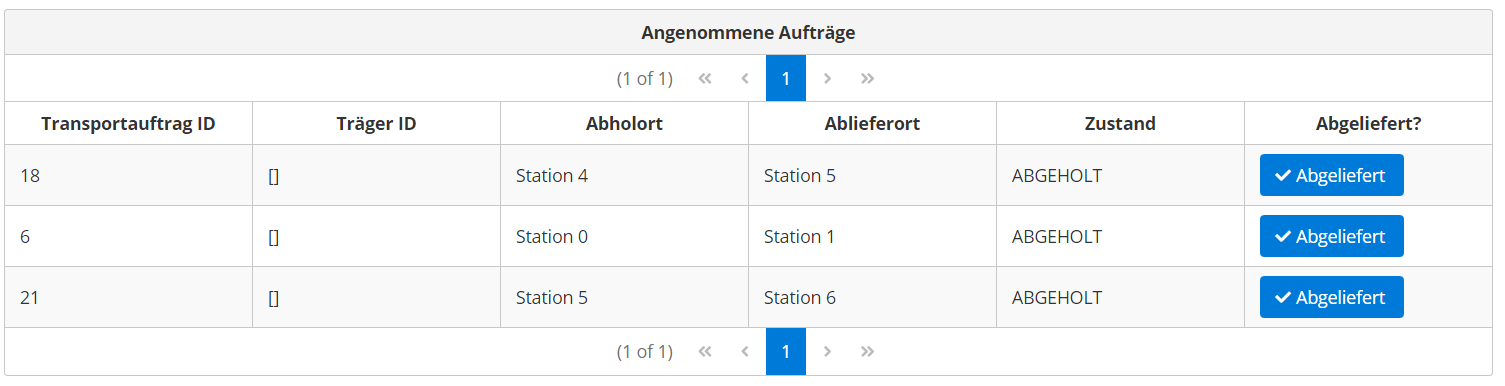
\includegraphics[width=\textwidth]{screenshots/tr/angenommen.png}
  \caption{Angenomme Transportaufträge}
  \label{fig:boat2}
\end{center}
\end{figure}


In der zweiten Tabelle stehen alle Aufträge, die aktuell verfügbar sind, also noch nicht von anderen Transportern angenommen wurden. Sie können einen Auftrag annehmen, indem Sie am Ende der entsprechenden Zeile auf Annehmen klicken. Dieser Auftrag ist dadurch nicht mehr für andere Transporter sichtbar, und erscheint nur in Ihrer Tabelle. \\

\begin{figure}[h!]
\begin{center}
 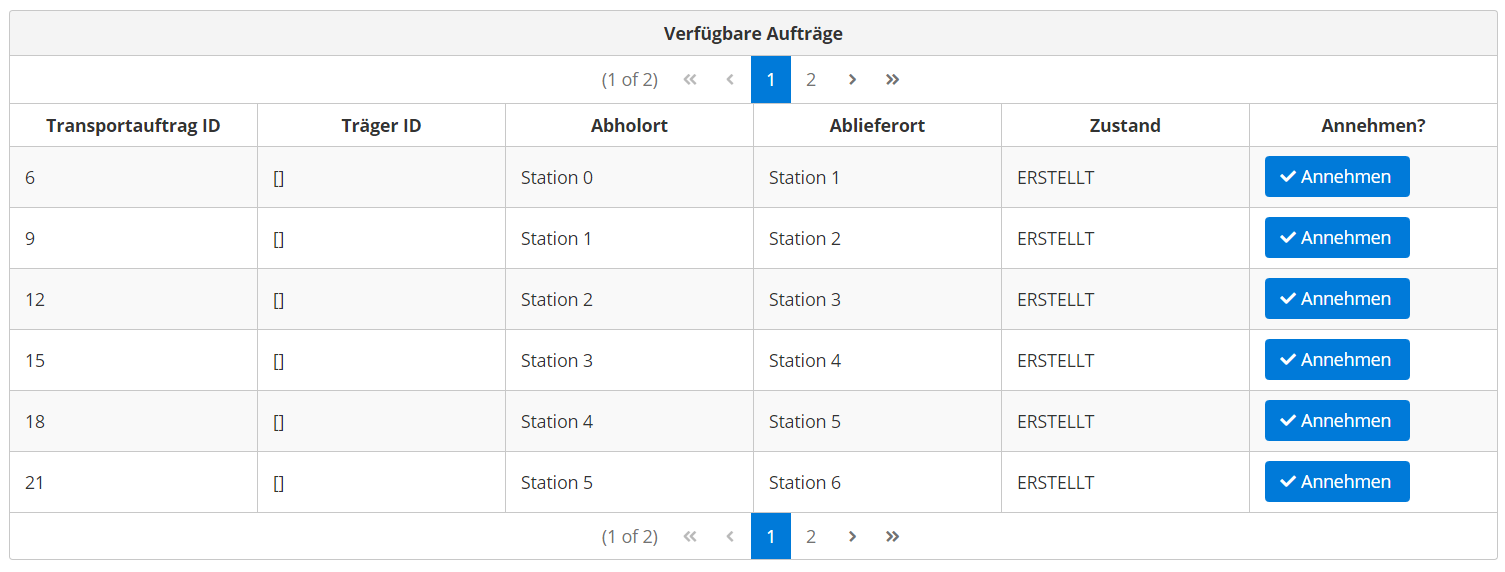
\includegraphics[width=\textwidth]{screenshots/tr/verfuegbar.png}
  \caption{Verfügbare Transportaufträge}
  \label{fig:boat2}
\end{center}
\end{figure}


In der unteren Tabelle sehen Sie Ihre alten Aufträge, die Sie bereits durchgeführt haben. Sie haben eine Übersicht über die Erstellungs-, Abholungs-, und Ablieferungszeit, und den aktuellen Zustand. An diesen Aufträgen können Sie keine Änderungen mehr vornehmen. \\

\begin{figure}[h!]
\begin{center}
 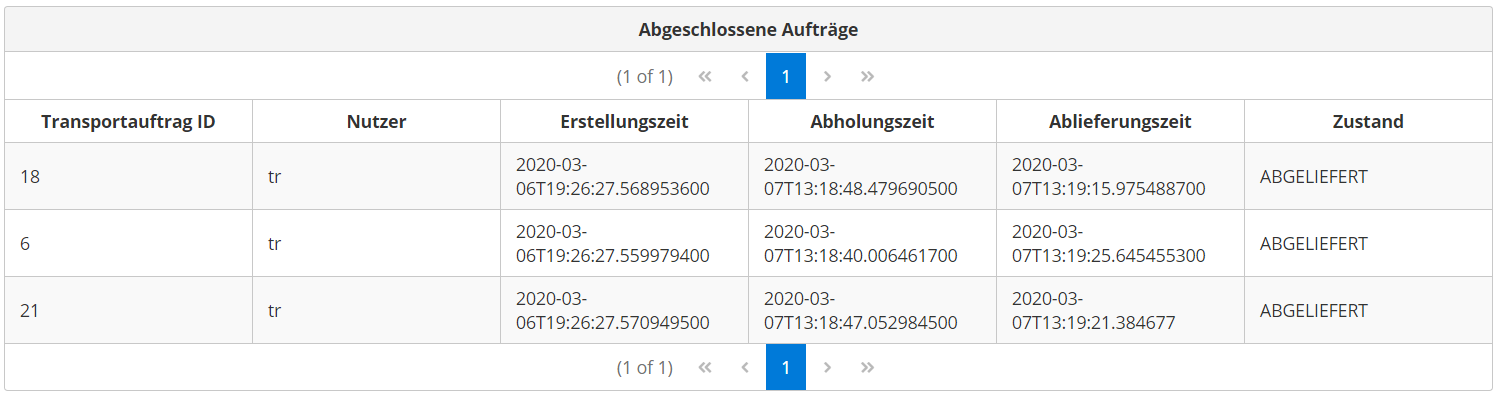
\includegraphics[width=\textwidth]{screenshots/tr/abgeschlossen.png}
  \caption{Abgeschlossene Transportaufträge}
  \label{fig:boat2}
\end{center}
\end{figure}


%%%%%%%%%%
\subsubsection{Probenverlust melden}
Im Menü-Unterpunkt Probenverlust melden können Sie Proben als verloren melden. Dafür geben Sie die Proben-ID der Probengruppe, zu der die Probe gehört, die Sie melden wollen, sowie die Anzahl an Proben aus dieser Gruppe, die Sie melden wollen, ein. Wenn Sie beide Angaben gemacht haben, drücken Sie auf Senden, um die Probe(n) zu melden. \\

\begin{figure}[h!]
\begin{center}
 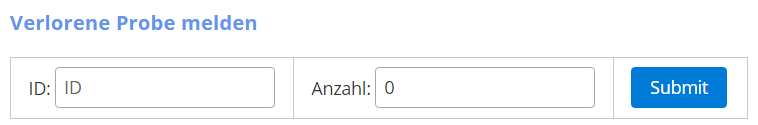
\includegraphics[width=\textwidth]{screenshots/tr/verloren.png}
  \caption{Probenverlust melden}
  \label{fig:boat2}
\end{center}
\end{figure}

\subsubsection{Fehler und Ursachen}
\begin{longtable}[c]{|p{5cm}|p{10cm}|}
\hline
\multicolumn{1}{|c|}{\textbf{Hinweis}}                          & \multicolumn{1}{c|}{\textbf{Ursache}}                                                                                                                                                                                                               \\ \hline
\endhead
Failed to start transport job! & Der Transportauftrag, den Sie annehmen wollen, konnte nicht in der Datenbank gefunden werden. \\ \hline
Failed to change state to Abgeliefert & Der Transportauftrag, dessen Status Sie ändern wollen, konnte nicht in der Datenbank gefunden werden.\\ \hline
\end{longtable}
%%%%%%%%%%%%%%%%%%%%%%%%%%%%%%%%%%%%%%%%%%%%%%%%%%%%%%%%%%%%%%%%%%%%%%%%

\newpage
\section{Referenz}
\subsection{Fehlermeldungen und Ursachen}
\subsubsection{502}
Wenn Sie die Fehlerseite .. sehen, ist ein Fehler im System aufgetreten. Bitte kontaktieren Sie das Entwicklerteam mit einer genauen Beschreibung der Vorgehensweise, der zum Auftreten dieses Fehlers geführt hat: Welche Seite haben Sie zuletzt besucht? Was haben Sie auf dieser Seite für eine Aktion ausgewählt? \\
Sie können zur Homepage zurückgehen, allerdings wird ein erneutes Laden der Seite die Aktion leider nicht für Sie ermöglichen, da es sich um einen tieferliegenden Fehler in der Implementierung handelt. \\

\begin{figure}[h!]
\begin{center}
 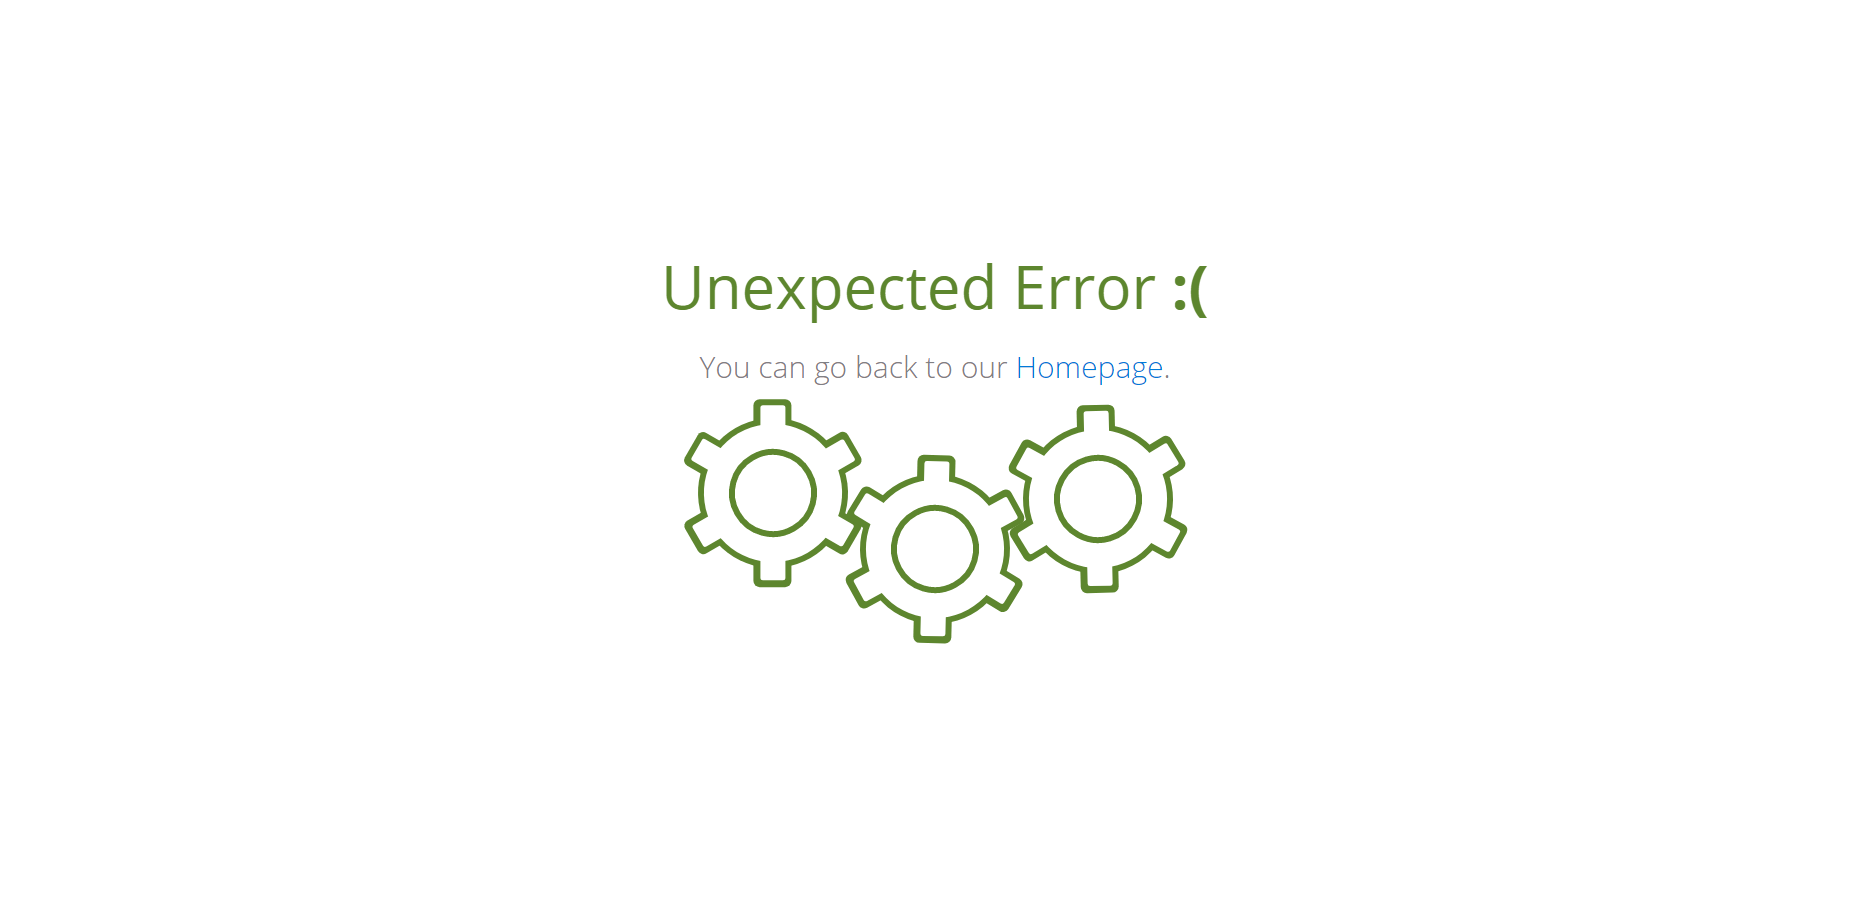
\includegraphics[width=\textwidth]{screenshots/allgemein/500.png}
  \caption{Fehler 502}
  \label{fig:boat1}
\end{center}
\end{figure}

\subsubsection{404}
Wenn Sie diese Fehlerseite sehen, versuchen Sie eine Seite aufzurufen, die nicht existiert. Bitte kontaktieren Sie das Entwicklungsteam mit einer genauen Beschreibung der Vorgehensweise, das zum Auftreten dieses Fehlers geführt hat. \\

\begin{figure}[h!]
\begin{center}
 
\includegraphics[width=\textwidth]{screenshots/allgemein/404.png}
  \caption{Fehler 404}
  \label{fig:boat1}
\end{center}
\end{figure}


\subsection{Index der Operationen}
\begin{longtable}[c]{|p{12cm}|p{3cm}|}
\hline
\multicolumn{1}{|c|}{\textbf{Operation}}                          & \multicolumn{1}{c|}{\textbf{Seite}}                                                                                                                                                                                                               \\ \hline
\endhead
Auftrag instanziieren & \\ \hline
Auftrag abbrechen & \\ \hline
Auftrag bearbeiten & \\ \hline
Auftrag starten  & \\ \hline
Auftrag Proben zuordnen & \\ \hline
Auftragsübersicht Logistiker & \\ \hline
Auftragsübersicht Transporter & \\ \hline
Auftragsübersicht Technologe & \\ \hline
Arbeitsauslastung  & \\ \hline
Benutzer bearbeiten & \\ \hline
Benutzer erstellen & \\ \hline
Benutzer löschen & \\ \hline
Erstinstallation & \\ \hline
Experimentierstation als kaputt melden & \\ \hline
Experimentierstation erstellen & \\ \hline
Experimentierstation löschen & \\ \hline
Experimentierstation bearbeiten & \\ \hline
Globale Einstellungen & \\ \hline
Lagerübersicht & \\ \hline
Probe als verloren melden & \\ \hline
Probenparameter hochladen  & \\ \hline
Proben erstellen  & \\ \hline //TODO
Prozesskettenvorlage erstellen & \\ \hline
Prozesskettenvorlagen bearbeiten & \\ \hline
Prozesskettenvorlagen löschen & \\ \hline
Prozessschritt Übersicht & \\ \hline
Prozessschritte als JSON exportieren  & \\ \hline
Aufträge als JSON exportieren & \\ \hline
Prozessschritt-Vorlage erstellen & \\ \hline
Prozessschritt-Vorlage löschen & \\ \hline
Prozessschritt-Vorlage bearbeiten & \\ \hline
Prozessschritt-Parameter erstellen & \\ \hline
Prozessschritt-Parameter löschen & \\ \hline
Prozessschritt-Parameter bearbeiten& \\ \hline
Prozessschritt-Parameter als JSON exportieren & \\ \hline
Prozessschritt-Zustandsautomat erstellen & \\ \hline
Prozessschritt-Zustandsautomat löschen & \\ \hline
Prozessschritt-Zustandsautomat bearbeiten & \\ \hline
Qualitative Eigenschaft erstellen & \\ \hline
Qualitative Eigenschaft löschen & \\ \hline
Qualitative Eigenschaft bearbeiten & \\ \hline
Quantitative Eigenschaft erstellen & \\ \hline
Quantitative Eigenschaft löschen & \\ \hline
Quantitative Eigenschaft bearbeiten & \\ \hline
Standort erstellen & \\ \hline
Systembackup & \\ \hline
Träger erstellen & \\ \hline
Träger löschen  & \\ \hline
Träger bearbeiten & \\ \hline
Transportauftrag annehmen  & \\ \hline

\end{longtable}

%%%%%%%%%%%%%%%%%%%%%%%%%%%%%%%%%%%%%%%%%%%%%%%%%%%%%%%%%%%%%%%%%%%%%%%%

\newpage
\section{Anhang}
\subsection{Glossar}
\begin{longtable}[c]{|p{7cm}|p{8cm}|}
\hline
\multicolumn{1}{|c|}{\textbf{Begriff}}                          & \multicolumn{1}{c|}{\textbf{Erklärung}}                                                                                                                                                                                                               \\ \hline
\endhead
Probe                                                           & Ein einzelner Werkstoff                                                                                                                                                                                                                              \\ \hline
Probengruppe						& Eine Gruppe an Proben, die die gleichen Eigenschaften haben. \\ \hline
Werkstoff                                                       & Mikrokugeln die sich durch Härte, hohe Belastbarkeit, Temperaturbeständigkeit und Abriebfestigkeit auszeichnen                                                                                                                                     \\ \hline
Träger                                                          & Transportmittel für Proben. Arten: Einzelträger, eingebettete Träger und Glasträger. Proben werden immer in Trägern transportiert                                                                                                                     \\ \hline
Experimentierstation \textbf{(ES)}             & Physischer Standort an dem Technologen Messungen durchführen.                                                                                                                                                                                     \\ \hline
Technologe                                                      & Ein Angestellter im SFB, er forscht und bedient die Experimentierstationen, und wertet diese im Anschluss aus und schreibt die Probeneigenschaften in die Software.                                                                                                  \\ \hline
Prozesskette \textbf{(PK)}                       & Besteht aus vielen Prozessschritten, die hintereinander ohne Verzweigung ablaufen. Sobald ein Auftrag erfolgt, wird eine Prozesskette gestartet.                                                                                                        \\ \hline
Prozesskettenauftrag \textbf{(PK-Auftrag)}     & Enthält die Prozessparameter für jeden Schritt einer Prozesskette. Der Prozesskettenadministrator legt die Prozessparameter fest. Der Logistiker legt die Proben und Träger fest.                                                                     \\ \hline
Prozessschritt \textbf{(PS)}                     & In einem Prozessschritt werden Werkstoffeigenschaften beeinflusst und / oder verändert. Er enthält Prozessparameter, welche beschreiben wie die Eigenschaften beeinflusst werden. Ein Prozessschritt kann Vorbedingungen haben und eine geschätzte Dauer. \\ \hline
Material- / Werkstoffeigenschaften                              & Jeder Werkstoff besitzt Eigenschaften. (Umformbarkeit / Verformbarkeit / ...)                                                                                                                                                                        \\ \hline
Prozessparameter \textbf{(PP)}                   & Sind qualitativ oder quantitativ. Qualitativ beschreibt, ob etwas so ist oder nicht. Quantitative Parameter enthalten einen Namen, ein Wert und eine Einheit.                                                                                          \\ \hline
Logistiker                                                      & Verwaltet das Archiv und alle Proben und Träger. Für die Ausführung einer Prozesskette bestimmt er welche Proben benutzt werden, falls dies nicht möglich ist, meldet er es dem Prozesskettenadministrator.                                           \\ \hline
Prozesskettenadministrator\textbf{ (PK-Admin)} & Verwaltet Prozessketten und deren Prozessschritte nach bestimmten Vorlagen. Verwaltet auch die Vorlagen. Ordnet Prozessschritten Experimentierstationen zu. Überprüft dann auf Korrektheit.                                                           \\ \hline
Transporter                                                     & Transportiert Träger mit ihren Proben zwischen Experimentierstationen. Bei Probenverlust meldet er diese.                                                                                                                                             \\ \hline
Transportauftrag \textbf{(T-Auftrag)}          & Enthält Start- und Zielexperimentierstationen, wird vom Transporter ausgeführt.                                                                                                                                                                      \\ \hline
System Administrator \textbf{(Sys-Admin)}      & Verwaltet Nutzer und Experimentierstationen. Konfiguriert globale Einstellungen und ist für Backups zuständig.                                                                                                                                         \\ \hline
Prozessketteninstanz Werte \textbf{(PIW)}      & Enthält für jeden Prozessschritt der Prozesskette alle Prozessparameter. Der Prozesskettenadmin benutzt die PIWs um Prozessketteninstanzen zu planen.                                                                                                 \\ \hline
Standort                                                        & Träger und Proben können entweder an einer Experimentierstation, im Archiv oder als verloren gemeldet sein.                                                                                                                                           \\ \hline
Transportauftragzustand \textbf{(TA-Zustand)}  & Ein Transportauftrag befindet sich im Zustand wartend oder er wurde schon geliefert.                                                                                                                                                                  \\ \hline
Prozessschrittzustand \textbf{(PS-Zustand)}    & Ein Prozessschrittzustand hat entweder den Zustand angenommen, in Bearbeitung oder abgegeben.                                                                                                                                                         \\ \hline
Upload in Datenbank                                             & Ein Technologe muss nach dem Ausführen eines Prozessschrittes die Prozessparameter in die Datenbank (DAVIS) hochladen.                                                                                                                                \\ \hline
\end{longtable}
\subsection{Index}

\end{document}